%%%%%%%%%%%%%%%%%%%%%%%%%%%%%%%%%% PREAMBULO %%%%%%%%%%%%%%%%%%%%%%%%%%%%%%%%%%%%%%

\documentclass[%
    %draft,%
    a4paper,%
    fontsize=12pt,%
    DIV=12,
    %oneside,%
    twoside,%
    openright,%
    titlepage=true,%
    headsepline,%
    toc=bibliography,%
    %
    parskip=half,%
    cleardoublepage=empty,%
    headings=big,%
]{scrbook}
\overfullrule=4ex


\usepackage[T1]{fontenc}%encoding de los fonts del pdf (para copiar y pegar)
\usepackage[utf8]{inputenc} %encoding del .tex
\usepackage{scrhack} %hacks para arreglar cosas de listings, babel, etc

\usepackage[spanish]{babel} %idioma español para los cortes de linea
\usepackage{amsmath} %paquete de matematica
% \usepackage[margin=2cm]{geometry} %margenes
\usepackage{enumerate} %mejor enumerate
\usepackage{xspace} %espacios despues de un comando
\usepackage{listings} %para escribir codigo C++
\usepackage{graphicx} % figuras
\usepackage{amsmath,amsthm,amssymb} %matematica
\usepackage{booktabs}%tablas bonitas
\usepackage{xspace}%espacios inteligentes
\usepackage{relsize}%para poder formatear bien C++ incluso en headers
\usepackage{tikz}%dibujos 
\usepackage{todo}%cosas para hacer
\usepackage[pdftitle={},pdfauthor={},pdfcreator={},pdfsubject={},pdfkeywords={},colorlinks=true,linkcolor=blue,citecolor=blue]{hyperref} %hiperlinks

\usetikzlibrary{external} 
\tikzexternalize 

%fuentes 
% \usepackage{palatino,mathpazo,eulervm}    %texto y matematica
\usepackage[scaled=0.8]{beramono} %codigo

\newtheorem{theorem}{Teorema}

\newcommand{\Grafo}{\textsc{Grafo}\xspace}
\newcommand{\Code}[2][]{\lstinline[basicstyle={\ttfamily},#1]@#2@}
\newcommand{\CPPCode}[2][]{\lstinline[language=C++,basicstyle={\ttfamily},#1]@#2@}
\newcommand{\N}{\mathcal{N}}
\newcommand{\Graph}{\CPPCode{Graph}\xspace}


\DeclareRobustCommand{\CPP}{C\nolinebreak[4]\hspace{-.05em}\raisebox{.4ex}{\relsize{-3}\textbf{++}}\xspace}
\pdfstringdefDisableCommands{%
  \def\CPP{C++}%
}
  
\lstset{
  numbers=left,
  numberstyle={\small\ttfamily},
  tabsize=2,
  frame=BRtl,
  basicstyle={\small\ttfamily},
  aboveskip={12pt},
  belowskip={12pt},
  captionpos=b,
  framerule=1.5pt,
  %linewidth=.9\linewidth
  xleftmargin=3em,
  xrightmargin=3em,
  emphstyle={\color{red}},
  escapechar=\%,
  breaklines=true,
  postbreak=\raisebox{2pt}[0ex][0ex]{\scriptsize\ensuremath{\hookrightarrow}}
}

\addtokomafont{caption}{\small}
\setkomafont{captionlabel}{\sffamily\bfseries}
\setcapindent{1em}
\setcapmargin{2em}

\renewcommand{\todomark}{Falta hacer:}
\renewcommand{\todoformat}{\color{red}\large\bfseries}

\begin{document}

%%%%%%%%%%%%%%%%%%%%%%%%%%%%%%%%%%% CARATULA %%%%%%%%%%%%%%%%%%%%%%%%%%%

\frontmatter
\begin{titlepage}

\vspace*{\stretch{1}}

\begin{center}

\includegraphics[width=9cm, keepaspectratio]{logo-unq.jpg}\\

\medskip

Departamento de Ciencia y Tecnología\\
Tecnicatura Universitaria en Programación Informática\\

\vspace{3cm}

\textbf{\huge Implementación de la estructura $h$-grafo}\\[0.4cm] 

\vspace{1.5cm}

{\large \bfseries \hspace{\stretch{3}}Griselda Cardozo\hspace{\stretch{1}}Alejandro Merlo\hspace{\stretch{3}}}

\end{center}

\vspace{3cm}

\textbf{Director:} Dr. Francisco Soulignac

\vspace{5mm}

Bernal, \today
\vspace*{\stretch{2}}
\end{titlepage}


\newpage

%%%%%%%%%%%%%%%%%%%%%%%%%%%%% RESUMEN %%%%%%%%%%%%%%%%%%%%%%%%%%%%

%Opcion para doble faz
\cleardoublepage

\vspace*{2cm}

\begin{center}
\Large \textbf{Implementación de la estructura $h$-grafo}
\end{center}

\vspace*{\stretch{1}}

En el presente trabajo implementamos la estructura $h$-grafo en el lenguaje de programación \CPP.  El objetivo principal de este trabajo es demostrar la viabilidad de la implementación en un lenguaje de programación real, usando su biblioteca estándar. Esta estructura se puede utilizar para resolver distintos problemas de grafos en tiempo $O(\alpha(G)|E(G)|)$, donde $\alpha(G)$ es la arboricidad de $G$.  Para verificar la corrección de la implementación, implementamos uno de estos algoritmos y comprobamos su eficiencia.

La estructura $h$-grafo representa a un grafo cualquier $G$ usando una lista de objetos, donde cada objeto \Code{v} representa a un vértice $v$ de $G$.  A su vez, cada objeto \Code{v} mantiene una lista \Code{L(k)}, que representa el $k$-vecindario de $v$ para $k \leq d(v)$, y una lista \Code{H}, que representa al vecindario alto de $v$.  En otras palabras, \Code{L(k)} mantiene un objeto \Code{w} por cada vecino $w$ de $v$ con grado $k < d(v)$, mientras que \Code{H} mantiene un objeto \Code{w} por cada vecino $w$ de grado $k \geq d(v)$.  A la vez, cada objeto \Code{w} de \Code{L(v)} y \Code{H} guarda distinos punteros que permiten ubicar rápidamente a \Code{v} y al objeto que representa a $v$ en las listas de vecinos de $w$.  Esto permite la eficiente inserción y la eliminación de vértices y aristas.

Una de las particularidades de nuestra implementación es que utilizamos iteradores (provistos por la biblioteca estándar de \CPP) para representar a los punteros del $h$-grafo.  La ventaja de usar iteradores es que nos permiten insertar y borrar objetos de los contenedores sin la necesidad de conocer la estructura interna de los mismos.  De la misma forma, nuestra estructura provee iteradores al usuario para que el mismo pueda manipular el $h$-grafo; estos iteradores siguen los lineamientos y conceptos del estándar de \CPP y por lo tanto son compatibles con la biblioteca estándar.  Como resultado podemos ocultar la estructura del $h$-grafo al usuario sin sacrificar su eficiencia.

\noindent \textbf{Palabras clave:} \textit{$h$-grafo, grafos ralos, arboricidad, implementación.}

\vspace*{\stretch{2}}
\newpage
%Opcion para doble faz
\cleardoublepage



%%%%%%%%%%%%%%%%%%%%%%%%%% DEDICATORIA Y AGRADECIMIENTOS %%%%%%%%%%%%%%%%%%%%%%

\vspace*{\stretch{1}}
{\raggedleft\emph{A mi familia y a todos aquellos me brindaron su ayuda en la tecnicatura.\\ Griselda Cardozo.}\par
            \emph{A mi familia.\\ Alejandro Merlo.}\par}
\vspace*{\stretch{1}}

%Opcion para doble faz
\cleardoublepage

% \chapter*{Agradecimientos}
% 
% \Todo{Escribir los agradecimientos a  quien corresponda, o eliminar la sección}
% 
% \hspace*{\stretch{1}} Fecha del dia del agradecimiento.
% 
% %Opcion para doble faz
% \cleardoublepage

\tableofcontents

\mainmatter

\chapter{Introducción}
\label{sec:introduccion}

Los grafos son estructuras abstractas que sirven para modelar distintos tipos de relaciones matemáticas.  Formalmente, un \emph{grafo} es un par $G = (V, E)$ donde $V$ es un conjunto (finito) de \emph{vértices} y $E$ es un conjunto formado por pares de vértices.  En términos matemáticos, los vértices son objetos cuya única propiedad es la de ser distinguibles; en la práctica, los vértices representan objetos de algún dominio de aplicación.  Los pares $(v,w)$ que pertenecen a $E$ son llamados \emph{aristas}, y su propósito es reflejar alguna relación entre $v$ y $w$.  Los grafos se usan para modelar relaciones de problemas reales en forma abstracta.  Por ejemplo, una red social se modela con un grafo que tiene un vértice por cada persona y una arista entre dos vértices para indicar que las personas son amigas.  La ventaja de utilizar grafos en lugar de los objetos que ellos modelan, es que tenemos acceso a una terminología común, de manera tal que podemos traducir los avances de una aplicación a otra.  De esta forma, podemos aprovechar la teoría de grafos para resolver problemas de áreas tan diversas como las matemáticas discretas, la infórmatica, las telecomunicaciones, la biología, la sociología, la filosofía, etc.~\cite{GrossYellen2006}.  La \emph{teoría de grafos} es la disciplina que se encarga del estudio de grafos, mientras que la teoría \emph{algorítmica} de grafos se encarga de los problemas computacionales asociados.

El objetivo del presente trabajo es implementar la estructura de datos $h$-grafo descripta por Lin et al.~\cite{LinSoulignacSzwarcfiterTCS2012}.   Como objetivos particulares de nuestro desarrollo, esperamos:
\begin{itemize}
  \item Verificar la correctitud de la misma.  Si bien el artículo describe la estructura con suficiente detalle, la misma no está implementada en un lenguaje de programación real.  En consecuencia, podrían haber detalles de implementación no detectados a la hora de describir la estructura.
  \item Analizar la dificultad de implementar la estructura en un lenguaje eficiente de escala industrial.  Como es común en los artículos de investigación teóricos, los investigadores suponen la existencia de ciertas tipos de datos (como las listas) con una interfaz apropiada a sus objetivos.  Sin embargo, las implementaciones reales de las mismas muchas veces distan de dicha interfaz ideal, lo que obliga a re-implementar estructuras básicas (e.g., re-implementar listas para tener acceso a la representación interna) o a resolver las discrepancias usando las estructuras ya existentes (e.g., utilizar \emph{iteradores} como si fueran punteros a los nodos de la representación).  En este trabajo tomamos la segunda opción.
\end{itemize}
Como objetivo futuro, que excede el alcance del trabajo realizado, sería deseable también analizar la eficiencia de la estructura de datos, tanto de forma aislada como en comparación con otras estructuras.

La estructura $h$-grafo se usa para implementar el \emph{tipo abstracto de datos} (TAD) \Grafo, que es una representación computacional del correspondiente objeto matemático.  De acuerdo a la interfaz que uno elija para operar con un grafo, es posible definir distintos tipos de TADs, con distintas características, que sean más o menos útiles para las distintas aplicaciones.  En particular, la estructura $h$-grafo fue concebida para aplicaciones que requieren grafos dinámicos.  Por \emph{dinámico} nos referimos a que la interfaz debe proveer operaciones eficientes para insertar y borrar vértices y aristas, a la vez que provee operaciones eficientes de consulta.  Es por este motivo que el TAD \Grafo que nosotros presentamos es consistente con el dinamismo requerido por las aplicaciones.  

La estructura $h$-grafo es una estructura general que se puede usar para representar a cualquier grafo.  Sin embargo, la estructura es particularmente eficiente en grafos \emph{ralos}, i.e., grafos con pocas aristas.  Existen distintas definiciones que dan cuenta de qué es un grafo ralo.  La definición más básica (y general) establece que un grafo es ralo cuando tiene $O(n)$ aristas, siendo $n$ la cantidad de vértices del grafo.  Si bien esta noción es útil, el resultado es que cualquier grafo no-ralo se puede convertir en un grafo ralo agregando suficiente vértices de grado bajo.  En muchas aplicaciones, estos vértices se pueden preprocesar eficientemente, lo que nos deja con un grafo no-ralo.  En particular, la estructura $h$-grafo requiere, para ser eficiente, que cualquier parte del grafo sea rala.  En otras palabras, la estructura es eficiente cuando todo subgrafo con $k$ vértices tiene $O(k)$ aristas.  Esta es la noción que nosotros vamos a considerar cuando decimos que un grafo es ralo.  En particular, Nash-Williams~\cite{Nash-WilliamsJLMS1964} observo que un grafo es ralo bajo esta noción precisamente cuando su arboricidad es baja.

Los objetivos específicos de este este trabajo son:
\begin{enumerate}
  \item describir una interfaz apropiada para el TAD \Grafo, siguiendo los usos y costumbres de nuestro lenguaje de implementación (\CPP),
  \item desarrollar el TAD grafo implementado con la estructura $h$-grafo, aprovechando la biblioteca estándar de nuestro lenguaje,
  \item aplicar la estructura para resolver algún problema típico de grafos, y usarlo para
  \item verificar que la eficiencia teórica coincide con la de nuestra implementación para algunos grafos.
\end{enumerate}
Como objetivo a futuro quedará el análisis de la estructura en aplicaciones reales de gran escala.

El presente documento esta organizado de la siguiente forma.  En el Capítulo~\ref{sec:tad grafo} describimos el TAD \Grafo, desde un punto de vista agnóstico con respecto al lenguaje, haciendo un repaso de su interfaz.  En el Capítulo \ref{sec:h-grafo} explicamos la estructura $h$-grafo, a la vez que describiremos los diferentes algoritmos que implementan las distintas operaciones del TAD \Grafo.  Este Capítulo también está presentado en forma independiente al lenguaje.  Luego, en el Capítulo~\ref{sec:c++}, nos centraremos en la implementación del TAD usando el lenguaje \CPP. Este capítulo está dividido en dos secciones. La primera, Sección~\ref{sec:c++:interfaz}, da cuenta de la interfaz del $h$-grafo siguiendo los lineamientos de \CPP. La segunda, Sección~\ref{sec:c++:estructura}, explica cómo se implementa la estructura en \CPP aprovechando la biblioteca estándar.  El Capítulo~\ref{sec:experimentación} presenta brevemente algunos resultados en los que medimos la eficiencia de la estructura $h$-graph.  Finalmente, el Capítulo~\ref{sec:final} presenta un breve resumen de lo logrado junto con las posibilidades de desarrollo a futuro.

\section{Preliminares}
\label{sec:definiciones}

Como mencionamos en la sección anterior, el objetivo central de este trabajo es implementar un TAD \Grafo que explote la estructura de datos $h$-grafo.  El TAD \Grafo es una representación computacional del objeto abstracto \emph{grafo}, que es el que se estudia en teoría de grafos.  En esta sección incluimos definiciones de la teoría de grafos que son necesarias para comprender nuestro trabajo (ver Figura~\ref{fig:definiciones} en donde se ejemplifican muchas de las definiciones de esta sección).

\begin{figure}[t]
\parindent=0pt\small
  \centering
  \tikzsetnextfilename{grafo}
  \begin{tikzpicture}%
    [vertex/.style={circle, draw=black, fill=black, minimum size=3mm, inner sep=0mm},
    edge/.style={thick}]

    \node [vertex,label=above:$v_3$] (top) at (0, 1.6) {};
    \node [vertex,label=below:$v_4$] (bottom) at (0, -1.6) {};
    
    \node [vertex,label=left:$v_1$]        (1) at (-3, 0) {};
    \node [vertex,label=above left:$v_2$]  (2) at (-1, 0) {};
    \node [vertex,label=above right:$v_5$] (3) at ( 1, 0) {};
    \node [vertex,label=right:$v_6$]       (4) at ( 3, 0) {};

    \draw [edge] (top) to (2);
    \draw [edge] (top) to (3);
    \draw [edge] (bottom) to (2);
    \draw [edge] (bottom) to (3);
    \draw [edge] (1) to (2);
    \draw [edge] (2) to (3);
    \draw [edge] (3) to (4);
  \end{tikzpicture}%

  \caption{Grafo $G$ con $V(G) = \{v_1,v_2,v_3,v_4,v_5,v_6\}$ y $E(G) =\{v_2v_1,\penalty0 v_2v_3,\penalty0 v_2v_4,\penalty0 v_2v_5,\penalty0 v_5v_3, \penalty0 v_5v_4, \penalty0 v_5v_6\}$.  El vértice $v_3$ tiene grado $2$ y su vecindario es $\{v_2,v_5\}$. La secuencia $v_1, v_2, v_3$ es un camino, mientras que $v_2,v_3,v_5,v_2$ es un ciclo.  El grafo $H$ con $V(H) = V(G)$ y $E(H) = \{v_2v_1, v_2v_3, v_2v_4, v_5v_6\}$ es un bosque que es subgrafo generador de $G$, i.e., $H$ es un bosque generador de $G$.  Como \{$H$, $J$\} es una partición en bosques de $G$, con $V(J) = V(G)$ y $E(J) = E(G) \setminus E(H)$, entonces $\alpha(G) \leq 2$.  Más aún, $\alpha(G) = 2$ porque $G$ no se puede particionar en un único bosque (ya que no es un bosque).}\label{fig:definiciones}
\end{figure}

%Definiciones matematicas
Un \emph{grafo} es un par $G = (V, E)$ donde $V$ es un conjunto finito de \emph{vértices} y $E$ es un conjunto de pares no ordenados, llamados \emph{aristas}.  Vamos a escribir $V(G)$ y $E(G)$ para denotar a $V$ y $E$, mientras que al par no ordenado formado por $v$ y $w$ lo vamos a escribir como $vw$.  Para cada $vw \in E$, decimos que $vw$ \emph{incide} tanto en $v$ como en $w$ y que, por lo tanto, $v$ y $w$ son \emph{vecinos} o \emph{adyacentes}.  El grado $d(v)$ de un vértice $v$ es la cantidad de vecinos que tiene $v$.  El $k$-vecindario de $v$ es el conjunto $N(v, k)$ de todos los vecinos de $v$ que tienen grado $k$, para algun $k \in \mathbb{N}$.  Obviamente, $N(v,k) = \emptyset$ para todo $k \geq n$.  Al conjunto $N(v)$ de todos los vecinos de $v$ lo llamamos, simplemente, su \emph{vecindario}; notar que $d(v) = |N(v)|$.

% Observar también que $N(v)$ (resp.\ $H(v)$) es la unión de todos los $k$-vecindarios de $v$ (resp.\ con $k \geq d(v)$), i.e., $N(v) = \bigcup_{i=0}^{n-1}N(v,k)$ y $H(v) = \bigcup_{i=d(v)}^{n-1}N(v,k)$.

Un grafo $G'$ es un \emph{subgrafo} de $G$ cuando $V(G') \subseteq V(G)$ y $E(G') \subseteq E(G)$.  Si $V(G') = V(G)$, entonces $G'$ es un subgrafo \emph{generador} de $G$, mientras que si $E(G') = \{vw \in E(G) \mid v,w \in V(G')\}$, entonces $G'$ es un subgrafo \emph{inducido} de $G$.  Sean $V \subseteq V(G)$, $E \subseteq E(G)$, $v \in V(G)$ y $vw \in E(G)$.  Para simplificar la notación de los algoritmos, vamos a escribir:
\begin{itemize}
  \item $G \setminus E$ para referirnos al subgrafo de $G$ generado por $E(G) \setminus E$, 
  \item $G \setminus V$ para referirnos al subgrafo de $G$ inducido por $V(G) \setminus V$, 
  \item $G - vw$ para referirnos a $G \setminus \{vw\}$, y 
  \item $G - v$ para referirnos a $G \setminus \{v\}$.
\end{itemize}
En otras palabras, $G \setminus E$ (resp.\ $G - \{vw\}$) se obtiene eliminando las aristas de $E$ (resp.\ la arista $vw$), mientras que $G \setminus V$ (resp.\ $G - v$) se obtiene eliminando los vértices de $V$ (resp.\ el vértice $v$) y las aristas que inciden en algún vértice de $V$ (resp.\ en $v$). Análogamente, escribimos $H + vw$ para indicar que $G = H - vw$ y, únicamente en caso en que $N(v) = \emptyset$, $H = G + v$ para indicar que $G = H - v$.  

Decimos que un grafo $G$ es \emph{$k$-degenerado} cuando todo subgrafo de $G$ tiene al menos un vértice de grado menor o igual a $k$.  La \emph{degeneración} de $G$ es el mínimo valor $d(G)$ tal que $G$ es $d(G)$-degenerado.  Para un vértice $v$, el \emph{vecindario alto} de $v$ es el conjunto $H(v)$ que contiene a todos los vecinos de grado al menos $d(v)$ lo llamamos el \emph{vecindario alto}.  Al valor $h(v) = |H(v)|$ lo llamamos el \emph{$h$-index} de $v$.  El \emph{$h$-index} de $G$ es el máximo $h(G)$ tal que hay al menos $h(G)$ vértices con $h(G)$-index mayor o igual a $h(G)$.

Un \emph{camino} de $G$ es una secuencia de vértices distintos $v_1, \ldots, v_k$ tal que $v_iv_{i+1} \in E(G)$ para todo $1 \leq i < k$.  Un ciclo es una secuencia $v_1, \ldots, v_k, v_1$ tal que $v_1, \ldots, v_k$ es un camino.  Los \emph{bosques} son aquellos grafos que no tienen ciclos.  La \emph{arboricidad} $\alpha(G)$ de un grafo $G$ es la mínima cantidad de bosques generadores en las que se puede particionar $E(G)$.  

El siguiente resultado relaciona los parámetros de cantidad de aristas, grado, $h$-index, degeneración y arboricidad para un grafo $G$.  Este resultado es importante, ya que guía las estrategias de los distintos algoritmos a fin de reducir la complejidad temporal para grafos ralos.

\begin{theorem}[e.g.~\cite{ChibaNishizekiSJC1985,LinSoulignacSzwarcfiterTCS2012}]
 Si $G$ es un grafo con al menos dos vértices y $\delta$ es el mínimo entre los grados de los vértices, entonces
 \begin{displaymath}
   \frac{\delta}{2} < \frac{|E|}{|V|-1} \leq \alpha(G) \leq d(G) \leq 2\alpha(G) \leq 2h(G) \leq 2\sqrt{2|E|} \\
 \end{displaymath}
\end{theorem}

Recordemos que consideramos que grafo es ralo cuando la densidad $|E(H)|/|V(H)|$ es pequeña para todo subgrafo $H$ de $G$.  Como mencionamos en la sección anterior, $G$ es ralo cuando su arboricidad es baja.  La veracidad de este hecho surge del siguiente teorema de Nash-Williams.

\begin{theorem}[\cite{Nash-WilliamsJLMS1964}]
  Si $G$ es un grafo con al menos dos vértices, entonces
  \[\alpha(G) = \max\left\{\frac{|E(H)|}{|V(H)|-1} \ \middle| \ H \text{ es subgrafo de }G \text{ con } |V(H)| > 1\right\}\]
\end{theorem}

Los últimos teoremas de esta sección reflejan una estrategia válida para trabajar con grafos ralos, que es la de revisar únicamente los vecindarios altos de algunos vértices, ignorando sus otros vecinos.

\begin{theorem}[\cite{LinSoulignacSzwarcfiterTCS2012}]
 Sea $e_1, \ldots, e_m$ un ordenamiento de las aristas de un grafo $G$ con $e_i = v_iw_i$.  Si $h_i(v)$ es el valor de $h(v)$ en el subgrafo generador de $G$ que contiene las aristas $e_1, \ldots, e_i$ (con $1 \leq i \leq m$), entonces
 \[\displaystyle \sum_{i=1}^{m}(h_i(v_i)+h_i(w_i)) \leq 4\alpha(G)m.\]
\end{theorem}

Intuitivamente, el teorema anterior indica que si se agregan las aristas a $G$ en el orden indicado pagando $O(h_i(v)+h_i(w))$ tiempo para la arista $v_iw_i$, entonces el tiempo total del algoritmo es $O(m\alpha(G))$.  Esta cota es importante para los algoritmos dinámicos donde se agregan aristas.  En la versión ``estática'', donde el grafo es conocido en forma completa de antemano, el costo es el mismo.

\begin{theorem}[\cite{LinSoulignacSzwarcfiterTCS2012}]
  Si $G$ es un grafo, entonces $\displaystyle \sum_{vw \in E(G)}(h(v)+h(w)) \leq 4\alpha(G)m.$
\end{theorem}

Estos dos resultados aplican, de manera análoga, cuando uno considera vértices en lugar de aristas.

\begin{theorem}[\cite{LinSoulignacSzwarcfiterTCS2012}]
 Sea $v_1, \ldots, v_n$ un ordenamiento de los vértices de un grafo $G$.  Si $h_i(v)$ es el valor de $h(v)$ en el subgrafo de $G$ inducido por $v_1, \ldots, v_i$ (con $1 \leq i \leq n$), entonces
  \[\displaystyle \sum_{i=1}^{n}\sum_{w \in N(v_i)}h_i(w) \leq 4\alpha(G)m.\]
\end{theorem}
%
\begin{theorem}[\cite{LinSoulignacSzwarcfiterTCS2012}]
  Si $G$ es un grafo, entonces, $\displaystyle \sum_{v \in V(G)}\sum_{w \in N(v)}h(w) \leq 4\alpha(G)m.$
\end{theorem}



\chapter{El tipo abstracto Grafo}
\label{sec:tad grafo}

\def\lstlistingname{Pseudocódigo}
 
El propósito de esta sección es presentar la interfaz del tipo abstracto \Grafo que implementaremos.  Cada instancia de este TAD es \emph{dinámica}, en el sentido que la instancia va mutando de acuerdo la inserción de vértices y aristas.  Asimismo, el TAD ofrece distintas operaciones de consulta, que están pensadas para poder recorrer eficientemente el vecindario de las distintas aristas del grafo.  Estas operaciones son muy útiles, por ejemplo, cuando uno quiere analizar la estructura ``local'' del grafo.  Es decir, cómo se conectan los vecinos de un vértice $v$ dado entre sí.  

Para describir la interfaz del TAD \Grafo, vamos a detallar cada una de las operaciones junto con sus propósitos y sus requerimientos (precondiciones).  Esta descripción será de alto nivel, tal y como se desarrolla en~\cite{LinSoulignacSzwarcfiterTCS2012}.  La idea de esta sección es fijar los conceptos necesarios para la posterior descripción de su implementación en el lenguaje \CPP.  Asimismo, mostraremos ejemplos  de uso de las distintas operaciones y describiremos la complejidad temporal esperada.  Obviamente, esta complejidad está en función de la implementación que se pospone al Capítulo~\ref{sec:h-grafo}.  

Recordemos que si bien los vértices de un grafo son elementos abstractos, los mismos se usan para representar entidades de aplicaciones reales.  Es común que estas entidades tengan alguna información propia que es requerida dentro de la aplicación.  Es por este motivo que el grafo permite asociar cierta información a cada vértice, lo que convierte al TAD \Grafo en un tipo paramétrico.  Específicamente, el TAD \Grafo almacena objetos de un tipo un tipo genérico \Code{elem}.

Por último, remarcamos que la interfaz que presentamos hace un uso extensivo de iteradores a fin de proveer una estructura de acceso y manipulación de los vértices y aristas del grafo.  En términos simples, un iterador \Code{it} presenta una secuencia $S$ de elementos de un conjunto soporte $C$ a través de dos operaciones básicas.  La primer operación permite acceder al \emph{primer} elemento de $S$, la segunda permite modificar \Code{it}, ``descartando'' el primer elemento de $S$ (vale remarcar que el conjunto soporte $C$ no cambia).  Cuando uno trabaja con tipos dinámicos, es posible que el conjunto  soporte $C$ cambie, lo que afecta a la secuencia $S$ y altera el comportamiento de \Code{it}.  En general, puede ocurrir una de dos opciones:
\begin{itemize}
  \item que \Code{it} quede en un estado \emph{inválido}, en cuyo caso cualquier uso de \Code{it} resultará en un error de ejecución; esto ocurre usualmente cuando se elimina de $C$ el primer elemento de $S$,
  \item que \Code{it} quede \emph{permutado}, en cuyo caso \Code{it} es válido, pero que la secuencia recorrida $S$ cambió más allá de lo esperable por la operación aplicada (e.g., obviamente que si se elimina de $C$ un elemento de $S$, el mismo no será recorrido); esta situación ocurre cuando se cambian propiedades de los objetos de $C$ que alteran el orden fundamental de recorrido de \Code{it} (e.g., si se recorren los vértices de acuerdo a su grado, el agregado de aristas puede modificar el orden del recorrido).  
\end{itemize}
Obviamente, el uso de iteradores inválidos está prohibido.  En cambio, uno puede usar un iteradores después que queda permutado.  Sin embargo, se desaconseja el uso de iteradores en recorridos que los permutan, ya que podría ocurrir que algunos elementos no se procesen o que algunos elementos se procesen más de una vez.  En cualquier caso, la validez dependerá del uso que uno quiera darle al iterador.

\section{\texorpdfstring{\Code{create_graph()}}{create\_graph()}}
\label{sec:tad grafo:create-graph}

Crea un objeto \Code{G} que representa un grafo $G$ de elementos \Code{elem}. Retorna un puntero \Code{G} al nuevo grafo creado. Este objeto guarda cierta información correspondiente a los vértices y sus vecinos. El \lstlistingname~\ref{lst:pseudo:create_graph} muestra cómo crear un grafo $G$ vacío.

\begin{description}
  \item [Propósito:] crea un \Code{G} sin vertices ni aristas.
  \item [Retorna:] un puntero \Code{G} al grafo $G$.
  \item [Complejidad temporal:]  $O(1)$.
\end{description}


\begin{lstlisting}[caption={Ejemplo de uso de \Code{create\_graph}},gobble=2,float=ht,label={lst:pseudo:create_graph},emph={create_graph}]
  G := create_graph()
\end{lstlisting}

\section{\texorpdfstring{\Code{insert_vertex(G, info)}}{insert\_vertex(G, info)}}
\label{sec:tad grafo:insert-vertex}

Modifica un objeto \Code{G} que representa un grafo $G$ a fin de representar el grafo $G + v$.  Al vértice $v$ se le puede asociar cierta información que está reflejada por el parámetro \Code{info}.  Retorna un \Code{vertex_iterador} \Code{v} que está posicionado en el vértice $v$ agregado.  Decimos que \Code{v} \emph{representa} o \emph{apunta} a $v$.  Este iterador \Code{v} debe usarse para interactuar con $G$ a fin de modificar sus propiedades.  Notar que el iterador \Code{v} es un objeto conocido sólo por \Code{G} y no es compartido con otras instancias del TAD \Grafo.  En particular, el uso de \Code{v} con otra instancia que no sea \Code{G} conduce a un comportamiento indefinido.

El \lstlistingname~\ref{lst:pseudo:insert_vertex} muestra cómo usar \Code{insert_vertex}.
  
\begin{description}
  \item [Parámetros:] \Code{G} representa un grafo $G$ e \Code{info} es cualquier objeto.
  \item [Propósito:] modifica \Code{G} para representar al grafo $G + v$.
  \item [Retorna:] un \Code{vertex_iterator} \Code{v} al vértice $v$.
  \item [Complejidad temporal:] O(1) (más la copia de la información).
\end{description}


\begin{lstlisting}[caption={Ejemplo de uso de \Code{insert_vertex} para imprimir ``aa''. Ver Sección~\ref{sec:tad grafo:vertex-iterator} para más información de \Code{vertex_iterator}.},gobble=2,float=ht,label={lst:pseudo:insert_vertex},emph={insert_vertex}]
  G := create_graph()
  v := insert_vertex(G, `a')
  w := insert_vertex(G, `a')
  for v in vertex_iterator(G):
      print get_info(v)
\end{lstlisting}


\section{\texorpdfstring{\Code{remove_vertex(G, v)}}{remove\_vertex(G, v)}}
\label{sec:tad grafo:remove-vertex}

Modifica un objeto \Code{G} que representa un grafo $G$ a fin de representar al grafo $G - v$.  Para ello, \Code{v} debe ser un \Code{vertex_iterator} que represente a $v$; el resultado de la operación está indefinido cuando \Code{v} no representa a un vértice de $G$.  Como resultado de esta operación, se invalidan aquellos iteradores que están relacionados con $v$.  Esto incluye a cualquier:
\begin{itemize}
  \item \Code{vertex_iterator} que apunte a $v$, 
  \item \Code{neighbor_iterator} o \Code{H_neighbor_iterator} asociado a $v$, y 
  \item \Code{neighbor_iterator} o \Code{H_neighbor_iterator} asociado a $w \in N(v)$ que apunte a $v$.
\end{itemize}
Asimismo, cualquier \Code{neighbor_iterator} o \Code{H_neighbor_iterator} al que aún le reste recorrer algún vecino de $v$ quedará permutado.
  
El \lstlistingname~\ref{lst:pseudo:remove_vertex} muestra cómo usar \Code{remove_vertex}.
  
\begin{description}
  \item [Parámetros:] \Code{G} representa un grafo $G$ y \Code{v} representa a $v \in V(G)$.
  \item [Propósito:] modifica \Code{G} para representar al grafo $G - v$.
  \item [Complejidad temporal:] $O(d(v)h(G))$; $O(|E(G)|\alpha(G))$ si se aplica a todos los vértices.
\end{description}


\begin{lstlisting}[caption={Ejemplo de uso de \Code{remove_vertex} para imprimir `b'. Ver Sección~\ref{sec:tad grafo:vertex-iterator} para más información de \Code{vertex_iterator}.},gobble=2,float=ht,label={lst:pseudo:remove_vertex},emph={remove_vertex}]
  G := create_graph()
  v := insert_vertex(G, 'a')
  w := insert_vertex(G, 'b')
  remove_vertex(G, v)
  for vt in vertex_iterator(G):
      print get_info(vt)
\end{lstlisting}


\section{\texorpdfstring{\Code{add_edge(G, v, w)}}{add\_edge(G, v, w)}}
\label{sec:tad grafo:add-edge}

Modifica un objeto \Code{G} que representa un grafo $G$ a fin de representar el grafo $G + vw$.   Para ello, \Code{v} y \Code{w} deben ser \Code{vertex_iterator} que representen a $v$ y $w$, respectivamente; el resultado de la operación está indefinido cuando \Code{v} o \Code{w} no representan a vértices de $G$.  Como resultado de esta operación, queda permutado cualquier \Code{neighbor_iterator} o \Code{H_neighbor_iterator} correspondiente a vecinos de $v$ o $w$.

El \lstlistingname~\ref{lst:pseudo:add_edge} muestra cómo usar \Code{add_edge}.

\begin{description}
  \item [Parámetros:] \Code{G} representa un grafo $G$, \Code{v} y \Code{w} representan a $v, w \in V(G)$, respectivamente.
  \item [Propósito:] modifica \Code{G} para representar un grafo $G + vw$.
  \item [Complejidad temporal:] $O(h(v) + h(w))$
\end{description}


\begin{lstlisting}[caption={Ejemplo de uso de \Code{add_edge} para imprimir 2. Ver Sección~\ref{sec:tad grafo:neighbor-iterator} para más información de \Code{neghbor_iterator}.},gobble=2,float=ht,label={lst:pseudo:add_edge},emph={add_edge}]
  G := create_graph()
  v := insert_vertex(G, 1)
  w := insert_vertex(G, 2)
  add_edge(G, v, w)
  for n in neighbor_iterator(v):
      print get_info(n)
\end{lstlisting}


\section{\texorpdfstring{\Code{remove_edge(G, v, w)}}{remove\_edge(G, v, w)}}
\label{sec:tad grafo:remove-edge}

Modifica un objeto \Code{G} que representa un grafo $G$ a fin de representar el grafo $G - vw$.  Para ello, \Code{v} y \Code{w} deben ser \Code{vertex_iterator} que representen a $v$ y $w$, respectivamente; el resultado de la operación está indefinido cuando \Code{v} o \Code{w} no representan a vértices de $G$.  Como resultado de esta operación, se invalidan todos los \Code{neighbor_iterator} o \Code{H_neighbor_iterator} asociados a $v$ o $w$ que apunten a $v$ o $w$.  Asimismo, queda permutado cualquier \Code{neighbor_iterator} o \Code{H_neighbor_iterator} correspondiente a vecinos de $v$ o $w$.

El \lstlistingname~\ref{lst:pseudo:remove_edge} muestra cómo usar \Code{remove_edge}.

\begin{description}
  \item [Parámetros:] \Code{G} representa un grafo $G$, \Code{v} y \Code{w} representan vértices adyacentes $v$ y $w$ de $G$, respectivamente.
  \item [Propósito:] modifica \Code{G} para representar al grafo $G - \{vw\}$.
  \item [Complejidad temporal:] $O(h(v) + h(w))$
\end{description}


\begin{lstlisting}[caption={Ejemplo de uso de \Code{remove_edge} para imprimir $3$.  Ver Sección~\ref{sec:tad grafo:neighbor-iterator} para más información de \Code{neghbor_iterator}.},gobble=2,float=ht,label={lst:pseudo:remove_edge},emph={remove_edge}]
  G := create_graph()
  v := insert_vertex(G, 1)
  w := insert_vertex(G, 2)
  x := insert_vertex(G, 3)
  add_edge(G, v, w)
  add_edge(G, v, x)
  remove_edge(G, v, w)
  for n in neighbor_iterator(v):
      print get_info(n)
\end{lstlisting}


\section{\texorpdfstring{\Code{add_vertex(G, info, N)}}{add\_vertex(G, info, N)}}
\label{sec:tad grafo:add-vertex}

Modifica un objeto \Code{G} que representa un grafo $G$ a fin de representar un grafo $H$ tal que $G = H - v$, donde la información de $v$ está reflejada en el parámetro \Code{info}.  Para construir $H$, \Code{N} debe ser una lista de \Code{vertex_iterator} de $G$, de forma tal que $N(v)$ en $H$ coincide con los vértices representados por \Code{N}.   Intuitivamente, \Code{add_vertex(G, info, N)} representa al grafo que se obtiene de agregar un nuevo vértice $v$ cuyo vecindario esta representado por \Code{N}.  Retorna un \Code{vertex_iterador} \Code{v} que representa al vértice $v$ agregado.  Como resultado de esta operación queda permutado cualquier \Code{neighbor_iterator} o \Code{H_neighbor_iterator} que recorra vértices de \Code{N}.

El \lstlistingname~\ref{lst:pseudo:add_vertex_with_N} muestra cómo usar \Code{add_vertex}.

\begin{description}
  \item [Parámetros:] \Code{G} representa un grafo $G$, \Code{info} es cualquier objeto y \Code{N} es una lista de \Code{vertex_iterator} de \Code{G} que representa al vecindario $N$.
  \item [Propósito:] modifica \Code{G} para representar un grafo $G + \{vw \mid w \in N\}$.
  \item [Retorna:] un \Code{vertex_iterator} \Code{v} al vértice $v$.
  \item [Complejidad temporal:] $O(d(v)h(G))$; $O(|E(G)|\alpha(G))$ si se aplica a todos los vértices.
\end{description}


\begin{lstlisting}[caption={Ejemplo de uso de \Code{add_vertex} para imprimir ``12''.},gobble=2,float=ht,label={lst:pseudo:add_vertex_with_N},emph={add_vertex}]
  G := create_graph()
  x := insertVertex(G, 1);
  y := insertVertex(G, 2);
  v := add_vertex(G, 3, {x, y})
  for w in neighbor_iterator(v):
      print get_info(w)
\end{lstlisting}


\section{\texorpdfstring{\Code{vertex_iterator(G)}}{vertex\_iterator(G)}}%iterador
\label{sec:tad grafo:vertex-iterator}

Provee de un \Code{vertex_iterador} que permite desplazarse a través de los vértices del objeto \Code{G} que representa un grafo $G$.  Además del recorrido, cada \Code{vertex_iterator} puede usarse para manipular el vértice que apunta de forma eficiente.  Tener en cuenta que el iterador se invalida si se elimina el vértice apuntado por él.  Las inserciones o remociones de otros vértices y aristas no tienen efectos en el iterador.

El \lstlistingname~\ref{lst:pseudo:vertex_iterator} muestra cómo usar \Code{vertex_iterator}.

\begin{description}
  \item [Parámetros:] \Code{G} representa un grafo $G$.
  \item [Propósito:] proveer al usuario de un mecanismo para iterar los vértices de $G$.
  \item [Retorna:] un \Code{vertex_iterador} \Code{i} que apunta al ``primer'' vértice de $G$.
  \item [Complejidad temporal:] $O(1)$; el recorrido de cada vértice cuesta $O(1)$ también.
\end{description}


\begin{lstlisting}[caption={Ejemplo de uso de \Code{vertex_iterator} para imprimir alguna permutación de la secuencia 1,2.},gobble=2,float=ht,label={lst:pseudo:vertex_iterator},emph={vertex_iterator}]
  G := create_graph()
  x := insertVertex(G, 1);
  y := insertVertex(G, 2);
  for v in vertex_iterator(G):
      print get_info(v)
\end{lstlisting}


\section{\texorpdfstring{\Code{neighbor_iterator(v)}}{neighbor\_iterator(v)}}%iterador
\label{sec:tad grafo:neighbor-iterator}

Provee de un iterador, llamado \Code{neighbor_iterator}, que permite recorrer los vecinos del vértice $v$ representado por el \Code{vertex_iterator} \Code{v}.  De esta forma se puede acceder eficientemente a cada vecino de $v$.  Decimos que el iterador está \emph{asociado} a $v$, mientras que apunta a un vértice $w \in N(v)$ correspondiente a la posición actual del iterador.  Si bien no está implementado en esta versión, un \Code{neighbor_iterator} también podría usarse para eliminar directamente la arista entre $v$ y $w$, donde $w$ es el vértice apuntado por el iterador.  Tener en cuenta que el \Code{neighbor_iterator} asociado a $v$ que apunta a $w$ se invalida cuando se elimina $vw$.  Más aún, las operaciones que alteren a $N(v) \cup N(w)$ (i.e., inserciones y remociones de vecinos de $v$ o $w$) pueden dejar al iterador permutado.

El \lstlistingname~\ref{lst:pseudo:neighbor_iterator} muestra cómo usar \Code{neighbor_iterator}.

\begin{description}
  \item [Parámetros:] \Code{v} representa un vértice $v$.
  \item [Propósito:] proveer al usuario de un mecanismo para iterar los vecinos de $v$.
  \item [Retorna:] un \Code{neighbor_iterator} \Code{w} para recorrer $N(v)$.
  \item [Complejidad temporal:] $O(1)$; el recorrido de cada vecino cuesta $O(1)$ también.
\end{description}


\begin{lstlisting}[caption={Ejemplo de uso de \Code{neighbor_iterator} para imprimir un permutación de 1,2.},gobble=2,float=ht,label={lst:pseudo:neighbor_iterator},emph={neighbor_iterator}]
  G := create_graph()
  x := insertVertex(G, 1);
  y := insertVertex(G, 2);
  v := add_vertex(G, 3, {x, y})
  for w in neighbor_iterator(v):
      print get_info(w)
\end{lstlisting}


\section{\texorpdfstring{\Code{H_neighbor_iterator(v)}}{H\_neighbor\_iterator(v)}}%iterador
\label{sec:tad grafo:H-neighbors}

Provee de un iterador, llamado \Code{H_neighbor_iterator}, que permite recorrer $H(v)$ para el vértice $v$ representado por el \Code{vertex_iterator} \Code{v}.  De esta forma se puede acceder eficientemente a cada vecino ``alto'' de $v$.  Decimos que el iterador está \emph{asociado} a $v$, mientras que \emph{apunta} a un vértice $w \in H(v)$ correspondiente a la posición actual del iterador.  Si bien no está implementado en esta versión, un \Code{H_neighbor_iterator} también podría usarse para eliminar directamente la arista entre $v$ y $w$, donde $w$ es el vértice apuntado por el iterador.  Tener en cuenta que el \Code{H_neighbor_iterator} asociado a $v$ que apunta a $w$ se invalida cuando se elimina $vw$.  Más aún, las operaciones que alteren a $N(v) \cup N(w)$ (i.e., inserciones y remociones de vecinos de $v$ o $w$) pueden dejar al iterador permutado.

El \lstlistingname~\ref{lst:pseudo:H_neighbors} muestra cómo usar \Code{H_neighbor_iterator}.


\begin{description}
  \item [Parámetros:] \Code{v} representa un vértice $v$.
  \item [Propósito:] proveer al usuario de un mecanismo para iterar los vecinos de grado al menos $d(v)$.
  \item [Retorna:] un iterador \Code{i} apuntando al ``primer'' vértice de $H(v)$.
  \item [Complejidad temporal:] $O(1)$; el recorrido de cada vecino cuesta $O(1)$ también.
\end{description}


\begin{lstlisting}[caption={Ejemplo de uso de \Code{H_neighbor_iterator} para imprimir 3.},gobble=2,float=ht,label={lst:pseudo:H_neighbors},emph={H_neighbors}]
  G := create_graph()
  x := insertVertex(G, 1);
  y := insertVertex(G, 2);
  v := add_vertex(G, 3, {x, y})
  for w in H_neighbor_iterator(x):
      print get_info(w)
\end{lstlisting}

\section{\texorpdfstring{\Code{degree(v)}}{degree(v)}}
\label{sec:tad grafo:degree}

Dado un \Code{vertex_iterator} \Code{v} que representa un vértice $v$ de un grafo $G$, devuelve el grado de $v$ en $G$.  El \lstlistingname~\ref{lst:pseudo:degree} muestra cómo usar \Code{degree}.


\begin{description}
  \item [Parámetros:] \Code{v} representando un vértice $v$.
  \item [Retorna:] $d(v)$.
  \item [Complejidad temporal:] O(1)
\end{description}


\begin{lstlisting}[caption={Ejemplo de uso de \Code{degree} para imprimir $2$.},gobble=2,float=ht,label={lst:pseudo:degree},emph={degree}]
  G := create_graph()
  x := insertVertex(G, 1);
  y := insertVertex(G, 2);
  v := add_vertex(G, 3, {x, y})
  print degree(v)
\end{lstlisting}



\chapter{La estructura \texorpdfstring{$h$}{h}-grafo}
\label{sec:h-grafo}

En esta sección describimos la estructura $h$-grafo que usamos para implementar el TAD \Grafo descripto en la Sección~\ref{sec:tad grafo}.  Esta estructura está diseñada para grafos ralos, i.e., grafos cuya arboricidad o $h$-index es baja.  Esto se ve reflejado en  las complejidades temporales esperadas, dado que las mismas dependen de la cantidad de aristas, el $h$-index y la arboricidad del grafo.  La descripción la hacemos a alto nivel tal como en el artículo que introduce la estructura~\cite{LinSoulignacSzwarcfiterTCS2012}.  La idea es explicar, a continuación, cómo está compuesta la estructura interna del $h$-grafo y luego detallar cada uno de sus operaciones.


La estructura $h$-grafo \Code{G} que representa a un grafo $G$ es simplemente un lista \Code{G.vertices} que tiene un objeto \Code{v} para cada vértice $v$ del grafo $G$.  Este objeto \emph{representa} a $v$ y mantiene la tripla $(d(v), \N(v), H(v))$, donde $\N(v)$ es la secuencia que se obtiene de eliminar los conjuntos vacíos de $N(v,1), \ldots, N(v, d(v)-1)$.  Recordemos que:   
\begin{itemize}
\item $d(v)$ es el grado de $v$, i.e., su cantidad de vecinos,
\item $N(v,k)$ es el $k$-vecindario de $v$, i.e., el conjunto de vecinos de $v$ que tienen grado $k$, y
\item $H(v)$ es el \emph{vecindario alto} de $v$, i.e., el conjunto de vecinos de $v$ que tienen grado al menos $d(v)$.
\end{itemize}
Asimismo, recordemos que nuestra implementación almacena cierta información asociada a cada vértice $v$.

La Figura~\ref{fig:h-grafo} muestra cómo se representa el $h$-grafo \Code{G} de $G$.  Obviamente, el objeto \Code{v} que representa a $v \in V(G)$ mantiene un número \Code{v.deg} para representar a $d(v)$ y un puntero \Code{v.info} para representar la información asociada a $v$. Para representar a $H(v)$ utiliza una lista doblemente enlazada \Code{v.high}.  Por último, para representar $\N(v)$, el $h$-grafo mantiene una lista doblemente enlazada \Code{v.low}, donde cada elemento \Code{v.low(k)} representa un $k$-vecindario $N(v,k)$.  En esta lista los $k$-vecindarios de $v$ aparecen ordenados de acuerdo al grado de sus elementos; observar que \Code{v.low(k)} no es necesariamente el $k$-ésimo elemento, ya que los $k$-vecindarios vacíos no se almacenan en \Code{v.low}.  Por último, cada objeto \Code{w} de alguna lista \Code{v.low(k)} $\cup$ \Code{v.high}, que representa a $w \in N(v)$, mantiene los punteros (iteradores, ver abajo) \Code{w.neighbor_pointer}, \Code{w.list_pointer} y \Code{w.self_pointer} tales que:
\begin{itemize}
  \item \Code{w.neighbor_pointer} apunta al objeto de \Code{G.V} que representa a $w$,
  \item \Code{w.list_pointer} apunta a la lista \Code{N} de \Code{w.low} $\cup$ \Code{w.high} que contiene al objeto \Code{v'} que representa a $v$, y
  \item \Code{w.self_pointer} apunta a la posición de \Code{v'} dentro de \Code{N}.  En otras palabras, \Code{w.self_pointer} apunta a la encarnación de $v$ en el vecindario de $w$.
\end{itemize}

\newcommand{\caja}[1]{\fbox{\!\scriptsize#1\!}}
\newcommand{\VV}[3]{v_{#1}\caja{#2}=\left\{\parbox{13cm}{\ensuremath{#3}}\right.}
\newcommand{\NNN}[1]{\mathcal{N}=\left\{\parbox{11.5cm}{\ensuremath{#1}}\right.}
\newcommand{\NNNEmpty}{\mathcal{N}=\emptyset}
\newcommand{\neigh}[5]{#1\caja{#2}: \mathtt{s}=#3, \mathtt{l}=#4, \mathtt{n}=#5}
\newcommand{\NN}[3]{\mathtt{N}(#1)\caja{#2}=[#3]}
\newcommand{\NH}[2]{\mathtt{H}\caja{#1}=[#2]}


\begin{figure}[ht]
\parindent=0pt\small
% \begin{center}

$\VV{1}{1}{\mathtt{d}=1\\
           \NNNEmpty\\
           \NH{7}{\neigh{v_2}{8}{10}{9}{2}}}$\\[2mm]
$\VV{2}{2}{\mathtt{d}=4\\
           \NNN{\NN{1}{9}{\neigh{v_1}{10}{8}{7}{1}},\\
                \NN{2}{11}{\neigh{v_3}{12}{17}{16}{3}, \neigh{v_4}{13}{20}{19}{4}}}\\
           \NH{14}{\neigh{v_5}{15}{28}{27}{5}}}$\\[2mm]
$\VV{3}{3}{\mathtt{d}=2\\
           \NNNEmpty \\
           \NH{16}{\neigh{v_2}{17}{12}{11}{2}, \neigh{v_5}{18}{25}{24}{5}}}$\\[2mm]
$\VV{4}{4}{\mathtt{d}=2\\
           \NNNEmpty \\
           \NH{19}{\neigh{v_2}{20}{13}{11}{2}, \neigh{v_5}{21}{26}{24}{5}}}$\\[2mm]
$\VV{5}{5}{\mathtt{d}=4\\
           \NNN{\NN{1}{22}{\neigh{v_6}{23}{30}{29}{6}} \\
                \NN{2}{24}{\neigh{v_3}{25}{18}{16}{3}, \neigh{v_4}{26}{21}{19}{4}}}\\
                \NH{27}{\neigh{v_2}{28}{15}{14}{2}}}$\\[2mm]
$\VV{6}{6}{\mathtt{d}=1\\
           \NNNEmpty \\
           \NH{29}{\neigh{v_5}{30}{23}{22}{5}}}$%
%
% \end{center}%

\caption{Estado de los objetos almacenados por un $h$-grafo para representar al grafo de la Figura~\ref{fig:definiciones}.  A la izquierda de cada signo $=$ se muestra un objeto representando al vértice $v_i$, para $i = 1, \ldots, 6$. La posición de cada uno de estos objetos en la memoria de la máquina se muestra en una caja; por ejemplo, el objeto representando a $v_1$ ocupa la celda 1 de la memoria.  La información que se mantiene para cada vértice se muestra a la derecha de su signo $=$.  Aquí también la posición de cada objeto en la memoria aparece en una caja, pero sólo para aquellos objetos que están apuntados por algún puntero.  Por ejemplo, el objeto \Code{H} correspondiente a $v_1$ ocupa la celda $7$.  Las letras $\mathtt{s}$, $\mathtt{l}$ y $\mathtt{n}$ representan a los \Code{self_pointer}, \Code{list_pointer} y \Code{neighbor_pointer}, respectivamente.} \label{fig:h-grafo}
\end{figure}

Como discutimos en la Sección~\ref{sec:introduccion}, uno de los objetivos del trabajo es utilizar las estructuras que provee la biblioteca estándar del lenguaje de implementación.  En particular, queremos utilizar el tipo lista que esta biblioteca provee.  Como parte de nuestra estructura, necesitamos almacenar punteros a los ``nodos'' de la lista.  Este es un inconveniente no menor, ya que no tenemos acceso a la estructura interna de la lista.  Sin embargo, observando el uso que se hace de dichos punteros, vemos que alcanza con que el tipo lista provea algunas funciones que permitan crear, borrar y mover los objetos (i.e., nodos) eficientemente, para lo cual no necesitamos conocer la estructura de la lista.  Cada lenguaje provee un mecanismo distinto para resolver este problema.  En el lenguaje que elegimos (\CPP), la solución es usar iteradores de la lista, ya que proveen esta interfaz de \emph{puntero restringido}.  

Bajo la misma filosofía de ocultamiento de la información, la estructura del tipo \Grafo está oculta al usuario.  En particular, los objetos de cada grafo son privados, en el sentido de que un usuario no pueden manipular estos objetos directamente.  En su lugar, el usuario modifica $v$ a través de un puntero que obtiene al insertar el vértice (ver Sección~\ref{sec:tad grafo:vertex-iterator}).  Siguiendo el ejemplo de la biblioteca estándar de \CPP, vamos a utilizar iteradores para proveer este comportamiento de puntero restringido.  Es decir, usamos iteradores para brindar acceso en $O(1)$ a los elemento sin mostrar la estructura interna al usuario.  Vamos a suponer que existe una operación \Code{vertex_iterator} que dado un objeto \Code{v} de \Code{G.vertices} crea un iterador \Code{it_v} que apunta a \Code{v}.  Luego, usando el operador \Code{it_v->X} podemos acceder al campo (o método) \Code{X} de \Code{v}.  Asimismo, suponemos la existencia de las funciones
\begin{itemize}
  \item \Code{v.neighbors()} que retorna un iterador a los vértices de \Code{G.vertices} que pertenecen a \Code{v.low} $\cup$ \Code{v.high}, y 
  \item \Code{v.H_neighbors()} que retorna un iterador a los vértices de \Code{G.vertices} que pertenecen a \Code{v.high}.
\end{itemize}

En el resto de esta sección describimos cómo implementar las operaciones principales del TAD \Grafo (ver Sección~\ref{sec:tad grafo}) usando la estructura $h$-grafo.  Para que quede claro que estamos usando la estructura $h$-grafo, vamos a escribir la signatura de cada operación \Code{oper(G, ...)} usando la notación punto, i.e., \Code{G.oper(...)} a fin de remarcar que tenemos acceso a la estructura interna de \Code{G}.  Asimismo, vamos a suponer la existencia de las siguientes funciones básicas sobre listas.  Vale remarcar que estas funciones existen en la biblioteca estándar de nuestro lenguaje de implementación.
\begin{itemize}
  \item \Code{L.append(what, pos = None)}: agrega \Code{what} inmediatamente atrás de la posición de \Code{L} apuntada por el iterador \Code{pos}.  Si \Code{pos = None}, entonces lo agrega al final.
  \item \Code{L.prepend(what, pos = None)}: agrega \Code{what} inmediatamente antes de la posición de \Code{L} apuntada por el iterador \Code{pos}.  Si \Code{pos = None}, entonces lo agrega al inicio.
  \item \Code{L.first()}: retorna un iterador al primer elemento de \Code{L}.
  \item \Code{L.last()}: retorna un iterador al último elemento de \Code{L}. 
  \item \Code{L.empty()}: indica si \Code{L} está vacía.
  \item \Code{L.erase(pos)}: elimina el elemento de \Code{L} apuntado por el iterador \Code{pos}.
  \item \Code{L.transfer(z)}: mueve el objeto apuntado por el iterador \Code{z} hacia el inicio de \Code{L}.  La lista que antes contenía a \Code{z} ya no lo contiene más.  Esta operación no inválida iteradores, aunque obviamente los permuta.
\end{itemize}

\section{\texorpdfstring{\Code{G.insert\_vertex(N = [], info = None)}}{G.insert\_vertex}}
\label{sec:hgraph:insert_vertex}

%IDEA

El proceso para insertar un nuevo vértice $v$ en $G$ se divide en dos partes.  Primero, se inserta un nuevo objeto \Code{v} que representa a $v$ en el grafo $H = G + v$.  Segundo, se inserta una arista $vw$ en $H$ para cada $w$ que este representado por uno de los objetos de $N$.  Claramente, el grafo $H$ así obtenido es tal que $N(v)$ se representa con \Code{N}.  El \lstlistingname~\ref{lst:pseudo:G.insert_vertex} muestra cómo está implementado \Code{insert_vertex}.

\begin{lstlisting}[caption={Implementación de \Code{insert_vertex}.},float=ht,label={lst:pseudo:G.insert_vertex}]
G.insert_vertex(N = [], info = None):
  v := G.vertices.append({deg = 0, high = [], low = [], info = info})
  for w in N:
    G.insert_edge(v, w)
  return vertex_iterator(v)
\end{lstlisting}

\section{\texorpdfstring{\Code{G.remove_vertex(v)}}{G.remove\_vertex(v)}}
\label{sec:hgraph:remove_vertex}

Para remover un vértice $v$ de $G$ revertimos el proceso de inserción.  Es decir, en primer lugar removemos las aristas que inciden en $v$ y luego eliminamos físicamente al objeto \Code{v} de \Code{G.vertices} que representa a $v$.  Para eliminar las aristas, se recorre el vecindario de $v$ y se aplica la función \Code{G.remove_edge(v,w)} (ver Sección~\ref{sec:hgraph:remove_edge}) para cada $w \in N(v)$.  El \lstlistingname~\ref{lst:pseudo:G.remove_vertex} muestra cómo está implementado \Code{remove_vertex}.

\begin{lstlisting}[caption={Implementación de \Code{remove_vertex}.},float=ht,label={lst:pseudo:G.remove_vertex}]
G.remove_vertex(v):
  for w in v->neighbors():
    G.remove_edge(v,w)
  G.vertices.erase(v)
\end{lstlisting}



\section{\texorpdfstring{\Code{G.insert_edge(v, w)}}{G.insert\_edge(v, w)}}
\label{sec:hgraph:insert_edge}

El algoritmo para insertar una nueva arista $vw$ al grafo $G$ (para $v, w \in V(G)$) tiene tres fases bien delimitadas que describimos a continuación.  En esta descripción suponemos que \Code{v} y \Code{w} son los \Code{vertex_iterator} que representan a $v$ y $w$.
\begin{description}
\item [Primer fase.] La primer fase consiste en actualizar los vecindarios de $v$ y $w$.  Recordemos que $H(v)$ contiene aquellos vecinos de $v$ que tienen grado al menos $d(v)$.  Como $d(v)$ se incrementa en $1$ cuando agregamos la nueva arista $vw$, estamos obligados a sacar de $H(v)$ aquellos vértices cuyo grado es exactamente $d(v)$.  Claramente, cada vértice $z \in H(v)$ que tenemos que sacar tiene grado $d(v)$.  Por lo tanto, tenemos que colocar todos estos vértices en un nueva lista \Code{N} que represente a $N(v, d(v))$.  Luego, para actualizar el vecindario de $v$, agregamos \Code{N} al final de \Code{v->low} y movemos cada \Code{z'} de \Code{v->high} con \Code{z->deg = v->deg} hacia \Code{N}, donde \Code{z = z'->neighbor_pointer} es el objeto que representa a $z$ en \Code{G.vertices}. Al mover \Code{z'}, tenemos que actualizar los iteradores asociados \Code{z'} y al objeto \Code{v'} que representa a $v$ en el vecindario de \Code{z}.  Tanto \Code{z'->neighbor_pointer} (que apunta a \Code{z}), como \Code{z'->list_pointer} (que indica la lista de \Code{z->low} $\cup$ \Code{z->high} donde se encuentra \Code{v'}) y \Code{z->self_pointer} (que indica la posición de \Code{v'} en \Code{z'->list_pointer}) son correctos.  Análogamente, \Code{v'->neighbor_pointer} es correcto y, si uno tiene cuidado de mover \Code{z'} sin invalidar los iteradores que lo apuntan, entonces \Code{v'->self_pointer} también es correcto.  En cambio, hay que actualizar \Code{v'->list_pointer} a fin de apuntar a la nueva lista \Code{N}.  Notemos que \Code{v'} se obtiene eficientemente accediendo a \Code{z'->self_pointer}.  Una vez actualizado el vecindario de $v$, se procede análogamente con $w$.  Es decir, agregamos la lista $N(w, d(w))$ a $\N(w)$ y movemos cada $z \in H(w)$ de grado $d(w)$ hacia $N(w, d(w))$.  Vale remarcar que $N(v,d(v))$ (resp.\ $N(w, d(w))$) se crea sólo si existe algún vecino de $v$ (resp.\ $w$) con grado $d(v)$ (resp.\ $d(w)$).  

\item [Segunda fase.]  La segunda fase consiste en actualizar el vecindario $N(z)$, para cada vértice $z$ que sea vecino de $v$ o $w$.  Notemos que si $v \in H(z)$ antes de la inserción, entonces $v \in H(z)$ luego de inserción, y por lo tanto el objeto \Code{v'} que representa a $v$ no debe actualizarse.  En cambio, si $v \not\in H(z)$, entonces $d(v) < d(z)$ en $G$ y $v \in N(z, d(v)) \in \N(z)$.  Por lo tanto, tenemos que mover \Code{v'} desde \Code{z->low(d(v))} hacia \Code{z->low(d(v)+1)} (o \Code{z->high} si \Code{v->deg + 1 = z->deg}) para todo \Code{z = z'->neighbor_pointer} tal que \Code{z'} pertenece a \Code{v->high}.  Notemos que \Code{v'} es el objeto apuntado por \Code{z'->self_pointer}.  Por lo tanto, podemos acceder eficientemente a \Code{v'} para moverlo.  Al igual que en la primer fase, tenemos que actualizar \Code{z'->list_pointer} para apuntar a la nueva lista que contiene a \Code{v'}.  Una vez finalizado el procesamiento de $H(v)$, tenemos que proceder de manera análoga con $H(w)$.
%
\item [Tercer fase.] Por último, tenemos que agregar físicamente a $vw$ en $G$.  Supongamos que $d(v) \leq d(w)$.  Primero creamos un objeto \Code{w'} en \Code{v->high} que represente a $w$.  Luego, buscamos la lista \Code{N} que representa a $N(w, d(v))$, recorriendo \Code{w->low} (si $d(v) < d(w)$) o tomando \Code{N = w->high} (si $d(v) = d(w)$).  Finalmente, insertamos un objeto \Code{v'} que represente a $v$ en $N(w)$ e  incrementamos \Code{v->deg} y \Code{w->deg} en $1$.  
\end{description}
El \lstlistingname~\ref{lst:pseudo:G.insert_edge} resume la implementación del algoritmo, mientras que la Figura~\ref{fig:insert_edge_después} muestra cómo queda la estructura de la Figura~\ref{fig:h-grafo} luego de insertar la arista $v_1v_6$. 

\begin{lstlisting}[caption={Implementación de \Code{insert_edge}.},float=ht,label={lst:pseudo:G.insert_edge}]
G.insert_edge(v,w):
  //Fase 1
  G.update_neighborhood(v); G.update_neighborhood(w)
  //Fase 2
  G.update_neighbors(v); G.update_neighbors(w)
  //Fase 3 (insercion fisica)
  if v->deg > w->deg: swap(v, w)
  if v->deg < w->deg: ubicar N := w->low(v->deg) recorriendo w->low
  else: N := w->high
  v' := N.prepend({neighbor_pointer=v})
  w' := v->high.prepend({neighbor_pointer=w})
  v'->self_pointer := N.first(); w'->self_pointer := v->high.first()
  v'->list_pointer := N; w'->list_pointer := v->high
  v->deg += 1; w->deg += 1

G.update_neighborhood(v):
  N := []
  for z' in v->high if v->deg = z'->neighbor_pointer->deg:
    N.transfer(z')
    //Obs: z'->self_pointer apunta a v dentro de z.high
    z'->self_pointer->list_pointer := N
  if not N.empty(): v->low.append(N)

G.update_neighbors(v):
  for z' in v->high if v->deg < z'->neighbor_pointer->deg:
    //Obs: z'->neighbor_pointer representa a z en G.vertices
    z = z'->neighbor_pointer
    //     z'->self_pointer representa a v en z->low,
    v' := z'->self_pointer
    //     y z'->list_pointer representa z->low(d(v))
    N_d := z'->list_pointer
     
    if v->deg + 1 < z->deg y z->low.next(N_d) != z->low(v->deg+1):
      N := z->low.append([], pos = N_d)
    if v->deg + 1 = z->deg:
      N := z->high
    N.transfer(v')
    if N_d = []: z->low.erase(N_d)
\end{lstlisting}

%%%%%%%%%%%%%%%%%%%%%%%%%%%%%%%%%%%%%%%%%%%%%%%%%%%%%%%%%%%%%%%%%%%%%%%%%



\begin{figure}[ht]
\parindent=0pt\small
% \begin{center}
$\VV{1}{1}{\mathtt{d}=2\\
           \NNNEmpty\\
           \NH{7}{\neigh{v_2}{8}{10}{11}{2}, \neigh{v_6}{31}{32}{29}{6}}}$\\[2mm]
$\VV{2}{2}{\mathtt{d}=4\\
           \NNN{\NN{2}{11}{\neigh{v_3}{12}{17}{16}{3}, \neigh{v_4}{13}{20}{19}{4}, \neigh{v_1}{10}{8}{7}{1}}}\\
           \NH{14}{\neigh{v_5}{15}{28}{27}{5}}}$\\[2mm]
$\VV{3}{3}{\mathtt{d}=2\\
           \NNNEmpty \\
           \NH{16}{\neigh{v_2}{17}{12}{11}{2}, \neigh{v_5}{18}{25}{24}{5}}}$\\[2mm]
$\VV{4}{4}{\mathtt{d}=2\\
           \NNNEmpty \\
           \NH{19}{\neigh{v_2}{20}{13}{11}{2}, \neigh{v_5}{21}{26}{24}{5}}}$\\[2mm]
$\VV{5}{5}{\mathtt{d}=4\\
           \NNN{\NN{2}{24}{\neigh{v_3}{25}{18}{16}{3}, \neigh{v_4}{26}{21}{19}{4}, \neigh{v_6}{23}{30}{29}{6}}}\\
                \NH{27}{\neigh{v_2}{28}{15}{14}{2}}}$\\[2mm]
$\VV{6}{6}{\mathtt{d}=2\\
           \NNNEmpty \\
           \NH{29}{\neigh{v_5}{30}{23}{24}{5}, \neigh{v_1}{32}{31}{7}{1}}}$%
%
% \end{center}%

\caption{Resultado de la inserción de la arista $v_1v_6$ al grafo de la Figura~\ref{fig:definiciones}, cuya estructura se muestra en la Figura~\ref{fig:h-grafo}.  Notar como el objeto $v_1\caja{10}$ se mueve de $N(1)\caja{9}$ hacia $N(2)\caja{11}$.  Como resultado de dicho movimiento, $N(1)\caja{9}$ es eliminado por quedar vacío. Además, tenemos que actualizar el puntero \Code{list_pointer} de $v_2\caja{8}$ para que apunte a $N(2)\caja{11}$.
} \label{fig:insert_edge_después}
\end{figure}

\section{\texorpdfstring{\Code{G.remove_edge(v, w)}}{G.remove\_edge(v, w)}}
\label{sec:hgraph:remove_edge}

El algoritmo para remover la arista $vw$ del grafo $G$ consiste en deshacer, en el orden inverso, las tres fases que usamos para su inserción (ver Seccion~\ref{sec:hgraph:insert_edge}).  Sean \Code{v} y \Code{w} los \Code{vertex_iterator} que representan a $v$ y $w$.

\begin{description}
\item[Deshacer tercer fase.] Recordemos que la tercer fase del proceso de inserción de $vw$ consiste en agregar físicamente la arista $vw$.  Luego, para deshacer la tercer fase tenemos que remover físicamente a $vw$ de $G$.  Supongamos, intercambiando $v$ con $w$ de ser necesario, que $d(v) \leq d(w)$, i.e., $w \in H(v)$.  El primer paso es recorrer \Code{v->high} hasta localizar al objeto \Code{w'} que representa a $w$.  En el segundo paso, usamos \Code{w'->list_pointer} y \Code{w'->self_pointer} para acceder y borrar al objeto que representa a $v$ en la lista \Code{w->low(d(v))} (o \Code{w->high} cuando $d(v) = d(w)$).  Por último, eliminamos \Code{w'} de \Code{v->high} y decrementamos \Code{v->deg} y \Code{w->deg} en $1$.

\item[Deshacer segunda fase.] Al igual que para la inserción, la segunda fase consiste en actualizar $N(z)$ para cada vértice $z$ que sea vecino de $v$ o $w$.  Obviamente, en este caso, la actualización refleja la remoción de $vw$.  Notemos que si $d(v) \geq d(z)$ luego de deshacer la tercer fase, entonces $v \in H(z)$ tanto antes como luego del borrado.  En consecuencia, no hace falta actualizar al objeto \Code{v'} que representa a $v$ en $N(z)$.  En cambio, si $d(v) < d(z)$, entonces tenemos que mover \Code{v'} desde \Code{z->low(d(v)+1)} (si $d(v)+1 < d(z)$) o \Code{z->high} (si $d(v)+1=d(z)$) hacia la lista \Code{z->low(d(v))}, donde \Code{z} el el objeto que representa a $z$ en \Code{G.vertices}.  Notemos que $z \in H(v)$ en este caso.  En consecuencia, obtenemos cada \Code{z = z'->neighbor_pointer} recorriendo \Code{v->high}.  Para obtener y mover a \Code{v'}, utilizamos \Code{z'->list_pointer} y \Code{z'->self_pointer} como en la segunda fase de la inserción.  Finalmente, actualizamos \Code{z'->list_pointer} para reflejar el movimiento.

\item[Deshacer primer fase.] En esta fase actualizamos el vecindario de $v$ y $w$, a fin de reflejar la remoción de $vw$.  Recordemos que en la primer fase de inserción de $vw$ movimos cada $z \in H(v)$  de grado $d(v)$ a una lista $N(v,d(v))$, debido a que $d(v)$ aumentaba en 1. Para deshacer este proceso, movemos cada vértice $z$ $\in N(v,d(v))$  hacia $H(v)$. Recordemos que en el $h$-graph cada lista $N(d(v))$ es una lista no vacía, razón por la cual $N(v,d(v))$ es finalmente eliminada.
\end{description}
El \lstlistingname~\ref{lst:pseudo:G.remove_edge} resume la implementación del algoritmo.


\begin{lstlisting}[caption={Implementación de \Code{remove_edge}.},name=remove_edge,gobble=2,float=ht,label={lst:pseudo:G.remove_edge}]
  G.remove_edge(v,w):
      if v->deg > w->deg: swap(v,w)
      //Deshacer Fase 3
      buscar w' tal que w'->neighbor_pointer = w en v->high
      w'->list_pointer->erase(w'->self_pointer)
      v->high.erase(w')
      v->deg -= 1; w->deg -= 1
      //Deshacer Fase 2
      G.update_neighbors_delete(v); G.update_neighbors_delete(w)
      //Deshacer Fase 2
      G.update_neighborhood_delete(v); G.update_neighborhood_delete(w)
  
  G.update_neighbors_delete(v):
    for z' en v->high:
      z := z'->neighbor_pointer
      v' := z'->self_pointer
      N := z'->list_pointer
      P := if v->deg + 1 = z->deg then prev(N) else z->low.last() 
      if P != z->low(d(v)): P := z->low.append([], P)
      P->transfer(z'->self_pointer)
      if N = [] and v->deg+1 < z->deg: z->low.erase(N)
      z'->list_pointer := P
  
  G.update_neighborhood_delete(v):
    if v->low.last() != v->low(v->deg): return
    for z' in v->low.last():
      v->high.transfer(z')
      //z'->self_pointer representa a v en N(z).
      z->self_pointer->list_pointer := v->high
    v->low.erase(v->low.last())
\end{lstlisting}


\chapter{Implementación en \CPP}
\label{sec:c++}

En esta sección vamos a describir todos los detalles de la implementación de la estructura $h$-grafo en el lenguaje \CPP.  Este capítulo imita la estructura de los Capítulos~\ref{sec:tad grafo}~y~\ref{sec:h-grafo}, salvo que se omite la implementación de los algoritmos.\footnote{Los mismos pueden encontrarse en el código \CPP que se adjunta a este documento.}  Primero describimos la interfaz pública (Sección~\ref{sec:c++:interfaz}) y luego la la estructura interna (Sección~\ref{sec:c++:estructura}).  


\section{Interfaz de \CPP}
\label{sec:c++:interfaz}

En esta sección describiremos la interfaz pública de la clase \Graph que implementa al TAD \Grafo usando la estructura $h$-grafo.  La interfaz pública de \Graph contiene, en lenguaje \CPP, las funciones que fueron descriptas en alto nivel en la Sección~\ref{sec:tad grafo}.
Tal cual se observa y explicita en las Secciónes~\ref{sec:tad grafo}~y~\ref{sec:h-grafo}, el usuario no tiene acceso directo a los objetos que representan a los vértices del grafo en la estructura interna, sino que accede a los mismos a través de \emph{punteros restringidos}.  Siguiendo la política de la biblioteca estándar de \CPP, estos punteros se representan usando iteradores.  Es deseable que estos iteradores se encuadren en la jerarquía estándar de iteradores de \CPP.

Debido a la importancia de los iteradores en la definición de la interfaz pública, en esta sección empezamos describiendo los tres tipos de iteradores que se proveen en este trabajo.  (Si bien no forma parte de este trabajo, es posible implementar otros iteradores, e.g. iteradores para recorrer y borrar aristas.)

\def\lstlistingname{Código}
\subsection{\texorpdfstring{\protect\CPPCode{Graph::vertex_iterator}}{Graph::vertex\_iterator}}
\label{sec:vertex iterator}

La clase \CPPCode{Graph::vertex_iterator}, o simplemente \CPPCode{vertex_iterator}, define los iteradores que apuntan al conjunto de los vértices del grafo.  Este iterador es el que se obtiene, por ejemplo, al aplicar las funciones \Code{vertex_iterator} (Sección~\ref{sec:tad grafo:vertex-iterator}) y \Code{add_vertex} (Sección~\ref{sec:tad grafo:add-vertex}).  Formalmente, la clase \CPPCode{vertex_iterator} implementa un iterador bidireccional constante de acuerdo a la jerarquía de \CPP.\footnote{Los iteradores bidireccionales permiten recorrer la estructura hacia adelante y atrás.  El iterador en todo momento apunta o bien a un vértice del grafo o bien a una posición indeterminada que representa el final de la secuencia iterada.  Al ser constante, el iterador no permite modificar la información asociada a un vértice.}  En consecuencia, su interfaz provee todas las funciones requeridas de este tipo de iteradores (e.g., \CPPCode{operator++} para avanzar, \CPPCode{operator--} para retroceder, etc.).  

Además de las funciones típicas de un iterador, la clase \CPPCode{vertex_iterator} provee las siguientes funciones que permiten acceder al vecindario del vértice $v$ apuntado por el iterador:
\begin{itemize}
 \item \CPPCode{operator*() const}: retorna la información asociada al vértice.
 \item \CPPCode{neighbor_iterator begin() const} y \CPPCode{neighbor_iterator end() const}: implementan la función \Code{neighbor_iterator} (ver Sección~\ref{sec:tad grafo:neighbor-iterator}) que permite recorrer el vecindario de $v$.  En particular, \CPPCode{begin} retorna un iterador al inicio de $N(v)$ (visto como una secuencia) y \CPPCode{end} retorna un iterador a la posición que le sigue al último elemento de $N(v)$.  La clase \CPPCode{neighbor_iterator} se describe en la Sección~\ref{sec:deg_iterator}. 
 \item \CPPCode{deg_iterator} \CPPCode{H_begin()} \CPPCode{const} y \CPPCode{deg_iterator} \CPPCode{H_end()} \CPPCode{const}: implementan la función \Code{H_neighbor_iterator} (Sección~\ref{sec:tad grafo:H-neighbors}) que permite recorrer los vecinos de grado al menos $d(v)$.  En particular, \CPPCode{begin} retorna un iterador al inicio de $H(v)$ (visto como una secuencia) y \CPPCode{end} retorna un iterador a la posición que le sigue al último elemento de $H(v)$.  El clase \CPPCode{deg_iterator} se describe en la Sección~\ref{sec:deg_iterator}. 
\end{itemize}

Hay dos formas para obtener una instancia de la clase \CPPCode{vertex_iterator}:
\begin{enumerate}[1.]
  \item Invocando el método \CPPCode{Graph::add_vertex}, que implementa la función \Code{add_vertex} (Sección~\ref{sec:tad grafo:add-vertex}) para agregar un nuevo vértice, e
  \item invocando alguno de los métodos \CPPCode{Graph::begin} o \CPPCode{Graph::end} que juntos implementan \Code{vertex_iterator} (Sección~\ref{sec:vertex iterator}).
\end{enumerate}
El \lstlistingname~\ref{lst:c++:const_vertex_iterator} muestra cómo usar un \CPPCode{vertex_iterator}.


\begin{lstlisting}[caption={Ejemplo de uso de \CPPCode{vertex_iterator} para manipular el grafo.  En el ejemplo, se crean dos vértices unidos por una arista y se imprimen los dos vértices.},name=const_vertex_iterator,gobble=2,float=ht,label={lst:c++:const_vertex_iterator},language=C++]
  void ejemplo_const_vertex_iterator() {
      Graph<int> G;
      Graph<int>::vertex_iterator v = G.insert_vertex(1);
      Graph<int>::vertex_iterator w = G.insert_vertex(2);
      //notar el uso de iteradores para agregar arista
      G.add_edge(v,w);

      for(auto it = G.begin(); it != G.end(); ++it) {
          cout << *it << endl;
      }
  }
\end{lstlisting}

\subsection{\texorpdfstring{\protect\CPPCode{Vertex::deg_iterator}}{Vertex::deg\_iterator} y \texorpdfstring{\protect\CPPCode{Vertex::neighbor_iterator}}{Vertex::neighbor\_iterator}}
\label{sec:deg_iterator}

La clase \CPPCode{Vertex::deg_iterator}, o simplemente \CPPCode{deg_iterator}, define los iteradores que permiten recorrer $H(v)$ para un vértice $v$. Este iterador es el que se obtiene, por ejemplo, al aplicar las función \Code{H_neighbor_iterator}\footnote{La razón por la cual la clase se llama \CPPCode{deg_iterator} en lugar de \CPPCode{H_iterator} es que esta clase se puede usar para recorrer $N(v, d)$ para cualquier grado $d < d(v)$ (de hecho, esa es una funcionalidad descrita en~\cite{LinSoulignacSzwarcfiterTCS2012}).  Sin embargo, no implementamos dicha funcionalidad en esta versión de forma pública.} (Sección~\ref{sec:tad grafo:H-neighbors}).  Análogamente, la clase \CPPCode{Vertex::neighbor_iterator}, o simplemente \CPPCode{neighbor_iterator}, define los iteradores que permiten recorrer $N(v)$; se obtienen, por ejemplo, al aplicar la función \Code{neighbor_iterator} (Sección~\ref{sec:tad grafo:neighbor-iterator}).  Formalmente, ambas clases proveen todas las funciones requeridas para ser considerados iteradores bidireccionales constantes de \CPP.

En principio, la única funcionalidad de ambos iteradores es poder acceder al vértice $w$ de $N(v)$ (o $H(v)$) que está siendo apuntado.  Hay dos opciones para implementar esta solución.  La primera, implementar el \CPPCode{operator*} a fin de que retorne un \CPPCode{vertex_iterator} que apunte a $w$.  La segunda, permitir el casteo automático desde \CPPCode{deg_iterator} y \CPPCode{neighbor_iterator} hacia \CPPCode{vertex_iterator}.  Para evitar múltiples indirecciones, elegimos la segunda opción, dejando el \CPPCode{operator*} como forma de acceder a la información asociada a $w$.  Además, cada iterador provee métodos para acceder al vecindario de $w$.  En resumen, se proveen las siguientes operaciones:
\begin{itemize}
  \item \CPPCode{operator*() const}: retorna la información asociada a $w$.
  \item \CPPCode{operator} \CPPCode{vertex_iterator()} \CPPCode{const}: casteo automático de un \CPPCode{deg_iterator} (o \CPPCode{neighbor_iterator}) a un \CPPCode{vertex_iterator} que apunta a $w$.
  \item \CPPCode{vertex_iterator as_vertex_iterator() const:} casteo explícito.
  \item \CPPCode{neighbor_iterator} \CPPCode{begin()} \CPPCode{const} y \CPPCode{neighbor_iterator} \CPPCode{end()} \CPPCode{const}: aplican \CPPCode{w->begin()} y \CPPCode{w->end()}, donde \CPPCode{w} es el \CPPCode{vertex_iterator} que apunta a $w$.   Conceptualmente, implementan la función \Code{neighbor_iterator} (Sección~\ref{sec:tad grafo:neighbor-iterator}) con parámetro $w$.
  \item \CPPCode{deg_iterator} \CPPCode{H_begin()} \CPPCode{const} y \CPPCode{deg_iterator} \CPPCode{H_end()} \CPPCode{const}:  \CPPCode{w->H_begin()} e \CPPCode{w->H_end()} donde \CPPCode{w} es el \CPPCode{vertex_iterator} que apunta a $w$. Conceptualmente, implementan la función \Code{H_neighbor_iterator} (Sección~\ref{sec:tad grafo:H-neighbors}) con parámetro $w$.  
\end{itemize}

Hay dos formas de obtener una instancia de las clase \CPPCode{deg_iterator}: 
\begin{enumerate}[1.]
  \item invocando \CPPCode{H_begin()} o \CPPCode{H_end()} sobre cualquier tipo de iterador (todos los iteradores a vértices incluyen esta función para evitar indirecciones), e 
  \item invocando \CPPCode{Graph::H_begin(v)} o \CPPCode{Graph::H_end(v)}, que toma un \CPPCode{vertex_iterator} \CPPCode{v} como parámetro.
\end{enumerate}
Análogamente, cambiando \CPPCode{H_begin} y \CPPCode{H_end} por \CPPCode{N_begin} y \CPPCode{N_end}, respectivamente, podemos obtener instancias de la clase \CPPCode{neighbor_iterator}.  El \lstlistingname~\ref{lst:c++:deg_iterator} muestra cómo usar estos iteradores.


\begin{lstlisting}[caption={Ejemplo de uso de \CPPCode{deg_iterator}.  En el ejemplo, se accede a $H(v)$ para un vértice $v$ invocando \Code{H_begin} usando el grafo, usando directamente un \Code{vertex_iterator} y usando un \Code{deg_iterator}.},name=deg_iterator,gobble=2,float=ht,label={lst:c++:deg_iterator},language=C++]
  //Imprime N(v)
  void print_high_neighborhood(const Graph<int>& G, vertex_iterator v) {
      for(auto it = G.H_begin(v); it != G.H_end(v); ++it) {
          //it es de tipo deg_iterator
          cout << *it << ',';
      }
  }
  
  //Para todo v, imprime los vertices de H(w) para w en H(v)
  void print_Ns_of_H(const Graph<int>& G) {
      for(auto v = G.begin(); v != G.end(); ++v) {
          //v es de tipo const_vertex_iterator
          for(auto w = v.begin(); w != v.end(); ++v) {
              //w es de tipo neighbor_iterator
              for(auto z = w.H_begin(); z != w.H_end(); ++z) {
                 //z pertenece a H(w) y w pertenece a H(v)
                 cout << *z << ',';
              }
          }
      }
  }
\end{lstlisting}

% \subsection{\Code{Vertex::neighbor_iterator}}
% \label{sec:neighbor iterator}
% \textbf{neighbor\_iterator}: es un iterador bidireccional que permite iterar todos los vecinos de un vértice. Es un iterador privado de la clase \textit{Vertex}. El usuario tiene acceso a él a través de la clase \textit{Graph} con los métodos \textit{N\_begin(const\_vertex\_iterator v))} y \textit{N\_end(const\_vertex\_iterator v))}
% 
%                         Ejemplo de uso del \textbf{neighbor\_iterator}
% \textit{}
%             \begin{lstlisting}[frame=single]
%             tip::Graph<int> G;
%             const_vertex_iterator v1 = G.insertVertex(1);
%             const_vertex_iterator v2 = G.insertVertex(2);
% 
%             for(auto it = G.N_begin(v1); it != G.N_end(v1); ++it) {
%                           cout << *it << ',';
%                       }
%             \end{lstlisting}

\subsection{Interfaz de la clase \texorpdfstring{\protect\CPPCode{Graph}}{Graph}}

Recordemos que el TAD \Grafo es un tipo paramétrico, ya que debe almacenar información arbitraria en los vértices.  En consecuencia, la clase \Graph es un \emph{template} que depende de un parámetro \CPPCode{Elem}.  Hay que tener en cuenta que las funciones que agregan vértices copian la información y, por lo tanto, las instancias de \CPPCode{Elem} deben ser copiables.  El resto de la interfaz pública se obtiene de traducir las operaciones del TAD \Grafo a \CPP usando los iteradores definidos en las secciones anteriores.  El \lstlistingname~\ref{lst:c++:graph_public} incluye las funciones principales de la interfaz de \CPPCode{Graph}.

\begin{lstlisting}[caption={Interfaz de la clase \CPPCode{Graph}.},gobble=2,name=graph_public,float=h,label={lst:c++:graph_public},language=C++,xleftmargin=1em,xrightmargin=1em]
  //add_vertex(*this, e) %(Sección~\ref{sec:tad grafo:insert-vertex})%
  vertex_iterator add_vertex(const Elem& e);
  
  //remove_vertex(*this, v) %(Sección~\ref{sec:tad grafo:remove-vertex})%
  void remove_vertex(vertex_iterator v);
  
  //add_edge(*this, v, w) %(Sección~\ref{sec:tad grafo:add-edge})%
  void add_edge(vertex_iterator v, vertex_iterator w);

  //remove_edge(*this, v, w) %(Sección~\ref{sec:tad grafo:remove-edge})%
  void remove_edge(vertex_iterator v, vertex_iterator w);
  
  //add_vertex(*this, e, N) y add_vertex(*this, e, N=[begin,end)) %(Sección~\ref{sec:tad grafo:add-vertex})%
  vertex_iterator add_vertex(const Elem& e, initializer_list<vertex_iterator> N)
  template<typename iter>
  vertex_iterator add_vertex(const Elem& e, iter begin, iter end);
  
  //vertex_iterator(*this) %(Sección~\ref{sec:tad grafo:vertex-iterator})%
  vertex_iterator begin() const;
  vertex_iterator end() const;

  //neighbor_iterator(*this, v) %(Sección~\ref{sec:tad grafo:neighbor-iterator})%
  neighbor_iterator N_begin(vertex_iterator v) const;
  neighbor_iterator N_end(vertex_iterator v) const;

  //H_neighbor_iterator(*this, v) %(Sección~\ref{sec:tad grafo:H-neighbors})%
  deg_iterator H_begin(vertex_iterator v) const;
  deg_iterator H_end(vertex_iterator v) const;
\end{lstlisting}




% Habiendo explicado las interfaces de los iteradores, estamos en condiciones de explicar la interfaz pública de la clase \textbf{Graph} que implementa las operaciones vistas en la Sección~\ref{sec:tad grafo}.  Remarcamos nuevamente que aquellos métodos que en la Sección~\ref{sec:tad grafo} requerían punteros toman iteradores como parámetro.  El tipo \textbf{Graph} provee los siguientes métodos:
% %
% \begin{itemize}
%   \item \Code{template<class iter> const_vertex_iterator add_vertex(const Elem& elem, iter begin, iter end)}: implementa la función \Code{G.insertVertex(N, info)} (Sección~\ref{sec:tad grafo:add-vertex}).  En este caso, \Code{this} se corresponde con \Code{G}, \Code{elem} con \Code{info}, y el rango \Code{[begin, end)} con \Code{N}.  Por otra parte, el puntero al nuevo vértice insertado es un \Code{vertex_iterator}.  Notar que se espera que el tipo \Code{iter} respete el protocolo de un iterador unidireccional de \CPP.
% \end{itemize}
% 
% 
% \subsubsection{insertVertex}
% \label{sec:insertVertex}
% \Code{insertVertex(const Elem\& elem)}: Su propósito es insertar un nuevo vértice al grafo.
% El tipo de retorno del método es un iterador \Code{const\_vertex\_iterator} (\ref{sec:vertex iterator}), recordemos que este iterador es el que va a permitir al usuario agregar y borrar aristas. El Codigo~\ref{lst:c++:insertVertex} muestra un ejemplo del uso.
% 
% \begin{lstlisting}[caption={Ejemplo de uso de insertVertex.  Crea un grafo $G$ de tipo entero con dos vértices, uno con el entero 1 y el otro con el entero 2 como información.  Luego, el ciclo imprime ``1 2''. Ver Sección~\ref{sec:vertex iterator} para más información de \texttt{vertex\_iterator}.},gobble=2,float=ht,label={lst:c++:insertVertex},emph={insert_vertex}]
%  
%   int main() {
%         Graph<int> G;
%         const_vertex_iterator v := G.insertVertex(1);
%         const_vertex_iterator w := G.insertVertex(2);
%         for(auto it = G.begin(); it != G.end(); ++it) {
%         cout << *it << endl;
%     }
%   }
% \end{lstlisting}
% 
% \subsubsection{remove\_vertex}
% \label{sec:remove-vertex}
% 
% \Code{remove\_vertex(const\_vertex_iterator v)}: Su propósito es eliminar un vértice \Code{v} del grafo y dejar en forma consistente el vecindario de los demás vértices con los que el vértice \Code{v} tenía relación. Esto significa eliminar las aristas que involucraban a \Code{v}.
% El método no tiene ningún tipo de retorno. El Codigo~\ref{lst:remove_vertex} muestra un ejemplo del uso.
% 
% \begin{lstlisting}[caption={Ejemplo de uso de remove\_vertex. Reescribimos el pseudocódigo ~\ref{lst:pseudo:remove_vertex} a c++. El código crea un grafo $G$ con dos vértices, el primero \texttt{v} representa al vértice $v$ con el número 1 y el segundo \texttt{w} representa al vértice $w$ con el número 2 como infomación. Luego, remueve \texttt{v} del grafo y el ciclo imprime ``2'' como resultado. Ver Sección~\ref{sec:vertex iterator} para más información de \texttt{vertex\_iterator}.},gobble=2,float=ht,label={lst:remove_vertex},emph={remove_vertex}]
%   int main() {
%         Graph<int> G;
%         const_vertex_iterator v := G.insertVertex(1);
%         const_vertex_iterator w := G.insertVertex(2);
%     remove_vertex(v);
%         for(auto it = G.begin(); it != G.end(); ++it) {
%         cout << *it << endl;
%     }
%  }
% \end{lstlisting}
% 
% 
% 
% \subsubsection{add\_edge}
% \label{sec:add-edge}
% \Code{add\_edge(const\_vertex\_iterator v, const\_vertex\_iterator w)}: Su propósito es crear la relación entre el vértice \Code{v} y el vértice \Code{w}. Deja en forma consistente el vecindario de \Code{v} y el vecindario de \Code{w}.
% 
% \subsubsection{remove\_edge}
% \label{sec:remove-edge}
% \Code{remove\_edge(const\_vertex\_iterator v, const\_vertex\_iterator w)}: su propósito es eliminar la relación entre los vértices \Code{v} y el vértice \Code{w}. Deja en forma consistente los vecindarios de los dos vértices.
% 
% Toma como parámetro un iterador que apunta a \Code(v) y otro que apunta a \Code{w}.
% 
% El método no tiene ningún tipo de retorno. El Codigo~\ref{lst:remove_vertex} muestra un ejemplo del uso.
% 
% \begin{lstlisting}[caption={Ejemplo de uso de \Code{remove_edge}.  Reescribimos el pseudocódigo ~\ref{lst:pseudo:remove_edge} a c++.  En el código se crea un grafo $G$ con vértices $v$, $w$ y $x$, siendo $v$ adyacente tanto a $w$ como a $x$.  Luego se utiliza \Code{remove_edge} para eliminar la arista $vw$, con lo cual $v$ queda adyacente únicamente a $x$.  El ciclo final, pues, imprime el valor $3$ asociado a $x$.  Ver Sección~\ref{sec:neighbor iterator} para más información de \Code{neighbor_iterator}.},gobble=2,float=ht,label={lst:remove_edge},emph={remove_edge}]
%   int main() {
%         Graph<int> G;
%         const_vertex_iterator v := G.insertVertex(1);
%         const_vertex_iterator w := G.insertVertex(2);
%     const_vertex_iterator x := G.insertVertex(3);
%     G.add_edge(v, w);
%     G.add_edge(v, x);
%     G.remove_edge(v, w);
%     for(auto it = G.N_begin(v); it != G.N_end(v); ++it) {
%         cout << *it << ',';
%     }
%   }
% \end{lstlisting}
% 
% 
% 
% 
% 
% 





\section{Estructura de representación en \CPP}
\label{sec:c++:estructura}

En esta sección describimos la estructura interna de la clase \Graph de \CPP que emula la estructura de un $h$-grafo vista en la Sección~\ref{sec:h-grafo}.  La implementación de estas estructuras se encuentra dividida en tres clases, cada una de las cuales se encuentra en su correspondiente archivo fuente:
\begin{itemize}
  \item \Code{Graph.h}: contiene la clase \CPPCode{Graph} que implementa la estructura principal del $h$-grafo.
  \item \Code{Vertex.h}: contiene la clase \CPPCode{Vertex} que contiene la descripción de lo que es un vértice.
  \item \Code{Neighbor.h}: contiene la clase \CPPCode{Neighbor} que representa lo que es un vecino de un vértice.
\end{itemize}
Las secciones siguientes describen las tres clases principales del $h$-grafo.

\subsection{Clase \texorpdfstring{\protect\CPPCode{Graph}}{Graph}}
\label{sec:c++:estructura:Graph.h}

Recordemos que el clase \Graph de \CPP es un \emph{template} que permite asociar información de algún tipo a cada vértice.  Como vimos en la Sección~\ref{sec:h-grafo}, la representación de un $h$-grafo es sencilla en términos conceptuales, ya que simplemente es una lista de vértices.  Esta lista está implementada con el tipo \CPPCode{std::list} y, dado que los vértices se implementan usando la clase \CPPCode{Vertex} (ver Sección~\ref{sec:c++:estructura:Vertex.h}), el tipo completo del miembro \CPPCode{vertices} es \CPPCode{std::list<Vertex>}.  La clase \Graph define también lo que es un \CPPCode{Graph::vertex_iterator}, que es una clase interna de \Graph.  

A pesar de la aparente simpleza, los tipos auxiliares (i.e., \CPPCode{Vertex} y \CPPCode{Neighbor}) deben estar al tanto de la estructura en la que se almacenan los vértices.  En efecto, cada instancia de \CPPCode{Neighbor} mantiene un iterador (\Code{neighbor_pointer}) que apunta a una posición de \CPPCode{vertices}.  Análogamente, cada instancia de \CPPCode{Vertex} necesita acceso al tipo paramétrico \CPPCode{Elem} de \Graph para saber qué tiene que guardar como información.  Para comunicar a las otras clases que \CPPCode{vertices} es de tipo \CPPCode{std::list}, hay al menos tres opciones.  La primera es copiar en cada clase los tipos no paramétricos (e.g., el tipo de \CPPCode{vertices}).  Esto no es muy flexible ya que, si la estructura cambiara\footnote{Por ejemplo para representar grafos estáticos conviene usar un \CPPCode{std::vector}.}, tendríamos que arreglar todos las clases auxiliares.  Una segunda opción es que las clases auxiliares sean \emph{templates} a fin de indicar los distintos parámetros que necesitan.  Una tercer opción más flexible es que las clases auxiliares sean \emph{templates} que dependan de la clase \CPPCode{Graph}.  De esta forma, podemos guardar todos los rasgos (\emph{traits}) en la clase \Graph.  Así, además de definir la estructura de \CPPCode{vertices}, la clase \CPPCode{Graph} contiene la definición de todos los renombres que son compartidos por las clases auxiliares (e.g., define el tipo donde se almacenan los vecindarios dentro de un vértice). En resumen, como veremos más adelante, las clases \CPPCode{Vertices} y \CPPCode{Neighbor} son \emph{templates} que se instancian como \CPPCode{Vertex<Graph>} y \CPPCode{Neighbor<Graph>}.  Más aún, la clase \Graph es \CPPCode{friend} de estas dos clases a fin de que puedan manipular la estructura interna. 

Volviendo un poco para atrás, la estructura de representación de \Graph está dada por \CPPCode{vertices} cuyo tipo, habíamos dicho, es \CPPCode{std::list<Vertex>}.  El inconveniente es que, de acuerdo al párrafo anterior, el tipo \CPPCode{Vertex} está incompleto, ya que \CPPCode{Vertex} es un \emph{template}.  Estrictamente hablando:
\begin{itemize}
  \item \CPPCode{vertices} es de tipo \CPPCode{std::list<Vertex<Graph<Elem>>>}
\end{itemize}
Esto no es un inconveniente para \CPP, ya que el tipo está bien definido más allá de que estemos definiendo la clase \Graph.  Queremos remarcar que, más allá del patrón de implementación, la estructura no deja de ser una lista de vértices.

El \lstlistingname~\ref{lst:c++:graph} muestra la estructura de la clase \Graph.

\begin{lstlisting}[language={C++},caption={Estructura del tipo Grafo en C++.},gobble=2,float=ht,label={lst:c++:graph}]
  template<class Elem> class Graph
  {
      using elem_type = Elem;
      //Vertex y Neighbor dependen de los rasgos de Graph<Elem>
      friend class Vertex<Graph>;
      friend class Neighbor<Graph>;
      using Vertex = Vertex<Graph>; 
      using Neighbor = Neighbor<Graph>;
      
      //Rasgos de Graph<Elem> que define todas las estructuras
      using Vertices = std::list<Vertex>;
      using degNeighborhood = std::list<Neighbor>;
      using Neighborhood = std::list<degNeighborhood>;
      using neighbor_iterator = typename Vertex::neighbor_iterator;
      using deg_iterator = typename Vertex::deg_iterator;

      //La estructura de representacion es una lista de vertices
      Vertices vertices;
  };
\end{lstlisting}

\subsection{Clase \texorpdfstring{\protect\CPPCode{Vertex}}{Vertex}}
\label{sec:c++:estructura:Vertex.h}

\CPPCode{Vertex} es la clase que define la estructura de un vértices del $h$-grafo.  De acuerdo a lo que discutimos en la Sección~\ref{sec:c++:estructura:Graph.h}, \CPPCode{Vertex} es \emph{template} con un parámetro que corresponde a clase \CPPCode{Graph} de la que forma parte.  Vale remarcar que el tipo \CPPCode{Vertex} se usa únicamente para la definición de clase \Code{Graph}, quien no exhibe la interfaz interna de \CPPCode{Vertex}.  En decir, la existencia de \CPPCode{Vertex} es invisible al usuario de \CPPCode{Graph}.  Por conveniencia, entonces, la estructura interna de \CPPCode{Vertex} es pública, ya que sólo define una estructura que igualmente es conocida por \Code{Graph}.

La clase \CPPCode{Vertex} posee la información asociada con el vértice $v$ (campo \CPPCode{elem}), el grado $d(v)$ del vértice (campo \CPPCode{degree}) y el vecindario $N(v)$ (campo \CPPCode{neighborhood}).  De acuerdo a lo discutido en la Sección~\ref{sec:h-grafo}, el vecindario en el $h$-grafo se almacena en una estructura especial con dos partes principales.  Por un lado, hay una lista de listas $\N$, que contiene cada una de las listas no vacías de $N(v, 0), \ldots, N(v, d(v)-1)$, en ese orden.  Por otro lado, se guarda una lista conteniendo los vértices de $H(v)$.  Recordemos que $N(v, i)$ contiene los vecinos de grado $i$, mientras que $H(v)$ contiene los vecinos con grado al menos $d(v)$.  Para la representación en \CPP, por comodidad, elegimos almacenar $H(v)$ como si fuera una última lista de $\N$.  En otras palabras, \CPPCode{neighborhood} es una lista de listas cuya última lista siempre representa a $H(v)$.

Recordemos que la clase \Code{Graph} concentra las definiciones de todos los tipos que forman la estructura.  Esto incluye qué estructura se usa para almacenar el vecindario $N(v)$ (tipo \CPPCode{Graph::Neighborhood}), qué estructura se usa para representar cada lista $N(v, i)$ y $H(v)$ dentro del vecindario (tipo \CPPCode{Graph::degNeighborhood}), y qué estructura se usa para representar un vecino del vecindario, i.e. el objeto que define el \CPPCode{self_pointer}, el \CPPCode{list_pointer} y el \CPPCode{neighbor_pointer} (tipo \Code{Graph::Neighbor}).  La clase \CPPCode{Graph} incluso define el tipo de vértice que se usa en \CPPCode{Graph::Vertex}.  Por comodidad, renombramos estos tipos dentro de la estructura de \CPPCode{Vertex}.  El \lstlistingname~\ref{lst:c++:vertex} muestra la estructura de \CPPCode{Vertex}.

\begin{lstlisting}[language={C++},caption={Estructura del tipo Vertex en \CPP.},gobble=2,float=ht,label={lst:c++:vertex}]
  template<class Graph> struct Vertex
  {
      //Tipo del elemento que se guarda en los vertice;
      //notar que es el tipo que el usuario indica en la clase Graph
      using elem_type = typename Graph::elem_type;
  
      //Estructura del vecindario, las listas internas y los vertices.
      using Neighborhood = typename Graph::Neighborhood;
      using degNeighborhood = typename Graph::degNeighborhood;
      using Vertices = typename Graph::Vertices;
      
      //Estructura del vertice
      elem_type elem;  //elemento
      size_t degree;  //grado
      Neighborhood neighborhood;  //vecindario
  };
\end{lstlisting}

\subsection{Clase \texorpdfstring{\protect\CPPCode{Neighbor}}{Neighbor}}
\label{sec:c++:estructura:Neighbor.h}

Las instancias de esta clase se usan para representar a las adyacencias en el grafo.  Supongamos que \CPPCode{G} representa a un grafo $G$ con dos vértices $v$ y $w$ que están representados por los objetos \CPPCode{v} y \CPPCode{w} en \CPPCode{G.vertices}.  Cuando $v$ y $w$ son adyacentes, una de las listas dentro de \CPPCode{v.neighborhood} contiene un objeto \CPPCode{w'} que representa a $w$ y, análogamente, una de las listas dentro de \CPPCode{w.neighborhood} contiene un objeto \CPPCode{v'} que representa a $v$.  Estos objetos \CPPCode{v'} y \CPPCode{w'} son instancias de la clase \CPPCode{Neighbor}.  

Como vimos en la Capítulo~\ref{sec:h-grafo}, la instancia \CPPCode{w'} debe mantener tres iteradores que se usan como punteros restringidos:
\begin{itemize}
  \item \CPPCode{w'.neighbor}: iterador a \CPPCode{G.vertices} que apunta a \CPPCode{w},

  \item \CPPCode{w'.list_pointer}: iterador a \CPPCode{w.neighborhood} apuntando a la lista \CPPCode{N} que contiene a \Code{v'},

  \item \CPPCode{w'.self_pointer}: iterador a \CPPCode{N} que apunta a \CPPCode{v'}.
\end{itemize}

Al igual que discutimos para la clase \CPPCode{Vertex}, la clase \CPPCode{Neighbor} también es un \emph{template} con un parámetro que debe corresponder con la clase \CPPCode{Graph} que lo utiliza.  Por comodidad, renombramos los tipos definidos dentro de la clase \CPPCode{Graph} dentro de \CPPCode{Neighbor}.  El \lstlistingname~\ref{lst:c++:neighbor} muestra la estructura interna de \CPPCode{Neighbor}.


\begin{lstlisting}[language={C++},caption={Neighbor.h},gobble=2,float=ht,label={lst:c++:neighbor}]
  template<class Graph> struct Neighbor
  {
      using NeighborPtr = typename Graph::Vertices::iterator;
      using SelfPtr = typename Graph::degNeighborhood::iterator;
      using ListPtr = typename Graph::Neighborhood::iterator;
      using elem_type = typename Graph::Vertex::elem_type;

      //Estructura para la arista vw dentro de v.neighborhood.
      //Para w' en v.neighborhood mantenemos:
      //- Puntero a w en G.vertices, 
      NeighborPtr neighbor;
      //- Puntero a la lista que tiene a v', 
      ListPtr list_pointer;
      //- Puntero a v'
      SelfPtr self_pointer;
  };
\end{lstlisting}

\chapter{Aplicaciones y experimentación}
\label{sec:experimentación}

El presente capítulo tiene dos propósitos prácticos que están relacionados.  Por un lado, queremos mostrar cómo se puede usar nuestra clase \CPPCode{Graph} para resolver un problema algorítmico de grafos que utiliza la estructura $h$-grafo.  El problema elegido en este caso es el computo de los triángulos del grafo.  Por el otro lado, queremos evaluar la eficiencia práctica de nuestra implementación para el problema propuesto.  El objetivo final de esta segunda parte es estudiar si el tiempo requerido por el algoritmo está en coincidencia con la cota teórica, a la vez que buscamos si el tiempo real de computo se asemeja más a la cota superior ($O(|E(G)|\alpha(G)$) o a la cota inferior ($\Omega(m)$).

\section{El problema de la búsqueda de triángulos}

Un \emph{triángulo} de un grafo $G$ es una tripla de vértices $\{v, w, z\}$ que son todos adyacentes entre sí.  El problema de \emph{listar los triángulos} consiste en enumerar todos los triángulos de un grafo de entrada $G$.  Este es un problema clásico de la teoría algorítmica de grafos que se resuelve usando distintos métodos.  Por ello, no podemos esperar que el grafo de entrada esté codificado usando un $h$-grafo, sino que viene descripto como el par $(V(G), E(G))$ donde $V(G)$ y $E(G)$ están implementados como listas o conjuntos.

En~\cite{LinSoulignacSzwarcfiterTCS2012} se propone un algoritmo para resolver el problema de listar los triángulos usando la estructura $h$-grafo.  Elegimos este algoritmo por dos razones principales.  Primero, porque es el más simple de implementar y, aún así, permite probar las características dinámicas de la implementación.  Segundo, porque este algoritmo coincide con una de las operaciones que en~\cite{LinSoulignacSzwarcfiterTCS2012} se incluyen como básicas para el resto de los algoritmos: la búsqueda de el conjunto $N'(v)$ de todas los aristas que junto a $v$ forman un triángulo.  Queda como trabajo a futuro la inclusión de esta operación dentro de la clase \CPPCode{Graph}.

Una vez construido el $h$-grafo de $G$, el algoritmo para listar los triángulos funciona considerando un vértice $v \in V(G)$ a la vez.  El primer paso es marcar cada vértice $z \in N(v)$.  Luego, se recorre cada $z \in H(w)$ para $w \in N(v)$: si $z$ está marcado, esto significa que $\{v,w,z\}$ es un triángulo; caso contrario, $\{v,w,z\}$ no es un triángulo porque falta la arista $vz$.  Para evitar duplicados, agregamos $\{v,w,z\}$ al resultado únicamente cuando $v$ es ``mayor'' a $w$ y $w$ es ``mayor'' a $z$ en algún sentido.  Una vez listados todos los triángulos correspondientes a $v$, borramos las marcas de los vértices en $N(v)$.  Este algoritmo cuesta $O(|E(G)|\alpha(G))$ tiempo~\cite{LinSoulignacSzwarcfiterTCS2012}.  El Pseudocódigo~\ref{lst:apps:triangulos-pseudo} muestra cómo implementar este algoritmo usando la interfaz descrita en el Capítulo~\ref{sec:tad grafo}, donde suponemos que existen las funciones \Code{marcar(z)}, \Code{marcado(z)} y \Code{desmarcar(z)} que, dado un \Code{vertex_iterator} \Code{z}, marca, verifica si está marcado, y desmarca a \Code{z}, respectivamente.

\def\lstlistingname{Pseudocódigo}
\begin{lstlisting}[caption={Algoritmo de búsqueda de triángulos, incluyendo la construcción del $h$-grafo.},gobble=2,float=ht,label={lst:apps:triangulos-pseudo}]
  listar_triangulos(V, E):
    listar_triangulos(construir_grafo(V, E))
    
  construir_grafo(V, E):
    G := create_graph()
    for v in V: it[v] := add_vertex(G, v)
    for (v,w) in E: add_edge(G, it[v], it[w])
  
  listar_triangulos(G):
    for v in vertex_iterator(G):
      for z in neighbor_iterator(G, v): marcar(z) 
      for w in neighbor_iterator(G, v):
        for z in H_neighbor_iterator(G, w):
          if marcado(z) and v > w > z: print {v, w, z}
      for z in neighbor_iterator(G, v): desmarcar(z)
\end{lstlisting}

\subsection{Implementación en \CPP}

Nuestra implementación en \CPP está igualmente dividida las dos fases principales: construir el $h$-grafo y listar los triángulos.  El algoritmo para listar los triángulos se incluye en el archivo \Code{triangles.h}.  La función principal llamada \CPPCode{triangles}, tiene un único parámetro de tipo \CPPCode{Graph<Marcable>}, donde \CPPCode{Marcable} es un tipo paramétrico.  La idea es que el objeto \Code{v} asociados al vértice $v$ del grafo pueda ser de cualquier tipo, siempre y cuando \Code{v} incluya dos funciones: \CPPCode{v.marcar(bool)} que se usa para marcar (cuando \CPPCode{bool} es verdadero) o desmarcar $v$ (cuando \CPPCode{bool} es falso).  Por otra parte, la función \CPPCode{triangles} retorna una lista de \CPPCode{Triangle<Marcable>}.  Cada instancia de \CPPCode{Triangle<Marcable>} mantiene tres \CPPCode{vertex_iterator}, uno por cada elemento del triángulo.  Asimismo, se incluye una función para determinar si un vértice es ``mayor'' a otro, a fin de evitar resultados duplicados.  (Para esta implementación, se requiere que los objetos que representan a los vértices, de tipo \CPPCode{Marcable}, sean también comparables.)  El Código~\ref{lst:apps:triangulos} muestra la implementación completa, excluyendo las funciones para determinar si un vértice es mayor a otro.  Podemos observar que, más allá de las características de los lenguajes, el Código~\ref{lst:apps:triangulos} es idéntico al presentado en el Pseudocódigo~\ref{lst:apps:triangulos-pseudo}.

\def\lstlistingname{Código}
\begin{lstlisting}[caption={Algoritmo de búsqueda de triángulos usando la clase \CPPCode{Graph}.},gobble=2,float=ht,label={lst:apps:triangulos}]
  template<class T>
  struct Triangle {
    typename Graph<T>::vertex_iterator v, w, z;
  };

  template<class Marcable>
  std::list<Triangle<Marcable>> triangles(const Graph<Marcable>& G) {
    std::list<Triangle<Marcable>> res;

    for(auto v = G.begin(); v != G.end(); ++v) {
      for(auto w = G.N_begin(v); w != G.N_end(v); ++w) w->marcar(true);

      for(auto w = G.N_begin(v); w != G.N_end(v); ++w)
        for(auto z = G.H_begin(w); z != G.H_end(w); ++z)
          if(z->marcado() && well_sorted(G, Triangle<Marcable>{v,w,z}))
              res.push_back(Triangle<Marcable>{v, w, z});
      
      for(auto w = G.N_begin(v); w != G.N_end(v); ++w) w->marcar(false);
    }
    return res;
  }
\end{lstlisting}

Si bien la construcción del objeto \CPPCode{Graph<Marcable>} \CPPCode{G} a partir de los conjuntos \CPPCode{V} y \CPPCode{E} no es compleja, hay dos detalles que conviene remarcar.  Primero, observemos que el parámetro de la función \CPPCode{triangles} es de tipo \CPPCode{const Graph<Marcable>&}, lo que significa que sus vértices no son modificables.  (En rigor, no incluimos ninguna función que permita cambiar la información de un vértice del grafo, que queda como trabajo futuro.)  En consecuencia, el mecanismo de la marcas se resuelve usando miembros mutables de \CPP.  El segundo detalle es cómo mantener la asociación entre los vértices de \CPPCode{V} y los iteradores que retorna el \CPPCode{G.add_vertex}.  La solución depende del uso que uno quiera darle a la clase \CPPCode{Graph}.  Una opción es guardar un diccionario que, dada una clave \CPPCode{v} de \CPPCode{V}, indique cuál es el iterador asociado.  Otra opción es usar números consecutivos entre $0$ y $|V|-1$ para representar a $V$, en cuyo caso se puede guardar un vector que asocie cada vértice con su iterador.  Nosotros tomamos esta segunda opción.  El Código~\ref{lst:apps:create_graph} muestra una posible implementación.


\begin{lstlisting}[caption={Una posible implementación de \CPPCode{construir_grafo}.},gobble=2,float=ht,label={lst:apps:create_graph}]
  struct Vertex {
    Vertex(int elem) : elem(elem), marked(false) {}
    ...
    int elem; mutable bool marked;
  };

  Graph<Vertex> construir_grafo(int n, std::list<std::pair<int,int>> E) {
    Graph<Vertex> G;
    vector<Graph<Vertex>::vertex_iterator> V;
    for(int v = 0; v < n; v++) V.push_back(G.add_vertex(v));

    for(auto e = E.begin(); e != E.end(); ++e)
       G.add_edge(V[e->first], V[e->second]);
    return G;  //se puede retonar V tambien.
  }
\end{lstlisting}

\section{Experimento}

El artículo~\cite{LinSoulignacSzwarcfiterTCS2012} contiene un análisis de la complejidad temporal del algoritmo de búsqueda de triángulos descrito en la sección anterior.  De acuerdo a este análisis, el algoritmo requiere tiempo $\Theta(|E(G)|\alpha(G))$, en peor caso, para encontrar los triángulos del grafo $G$ .\footnote{En rigor, el artículo~\cite{LinSoulignacSzwarcfiterTCS2012} indica que el costo es $O(|E(G)\alpha(G))$ para cualquier grafo.  Teniendo en cuenta que para algunas clases de grafos ---e.g., completos, árboles--- el costo es exactamente $O(|E(G)|\alpha(G))$, concluimos que en peor caso el costo es $\Theta(|E(G)|\alpha(G))$}  Recordemos que la arboricidad $\alpha(G)$ de $G$ coincide, en términos asintóticos, con la degeneración $d(G)$ de $G$.  Es decir, $\alpha(G) = \Theta(d(G))$, con lo cual podemos afirmar que el algoritmo cuesta $\Theta(|E(G)|d(G))$.  

El propósito de esta sección es comparar el tiempo de ejecución de nuestra implementación con el costo teórico esperado.  Nuestra expectativa es que, efectivamente, ambos tiempos coincidan, a fin de poder dilucidar (en forma experimental) dos preguntas complementarias.  Por un lado, ¿es cierto que el algoritmo propuesto en~\cite{LinSoulignacSzwarcfiterTCS2012}, que usa la estructura $h$-grafo, consume tiempo $O(|E(G)|\alpha(G))$?  Por otro lado, ¿es cierto que nuestra implementación cuesta $O(|E(G)|\alpha(G))$ tiempo?  Asimismo, aprovechamos la ejecución del algoritmo para testear que la implementación sea correcta.

Para la experimentación, generamos una serie de grafos usando el lenguaje de programación \Code{Python}.  Para cada grafo $G$ generado, realizamos las siguientes operaciones.
\begin{enumerate}
  \item En \Code{Python}, calculamos la degeneración $d(G)$ y el conjunto $T(G)$ de triángulos usando un algoritmo de fuerza bruta, que consiste en recorrer cada tripla $v,w,z$ de vértices, observando si son o no mutuamente adyacentes.  Codificamos el grafo en un archivo de texto plano, y guardamos $d(G)$ y $T(G)$ para el análisis futuro.
  \item Ejecutamos nuestro programa \CPP de calculo de triángulos usando el archivo generado, a la vez que medimos el tiempo $t(G)$ que consume el programa (medido en $\mu s$).  Como resultado obtenemos un conjunto de triplas $T'(G)$ que guardamos para el análisis futuro. 
  \item Nuevamente en \Code{Python}, comparamos $T(G)$ con $T'(G)$.  Si son iguales, concluimos que el algoritmo de \CPP es correcto para $G$; caso contrario, generamos un mensaje de error.
\end{enumerate}
Para crear los grafos de prueba, usamos distintos generadores provistos por la biblioteca \Code{networkx}~\cite{HagbergSchultSwart2008} de \Code{Python}.  Específicamente, generamos grafos completos (de hasta $60$ vértices), caminos (de hasta $19000$ aristas) y grafos aleatorios (mayormente ralos) usando las funciones: \Code{connected_watts_strogatz_graph}, \Code[mathescape]{erdos_$ $renyi_$ $graph}, \Code{gnp_random_graph}, \Code{newman_watts_strogatz_graph} y \Code[mathescape]{dense_$ $gnm_$ $random_$ $graph}.  Los grafos tienen entre $100$ y $20000$ aristas, y la degeneración de los mismos varía entre $1$ y $71$.

\section{Resultados del experimento}

Como resultado de nuestra experimentación, lo primero que observamos es que $T(G) = T'(G)$ para todos los grafos considerados.  Esto nos permite concluir, empíricamente, que el algoritmo es correcto para la gran cantidad de grafos analizados.  En consecuencia, es esperable que el algoritmo se comporte correctamente, aunque no hayamos descartado la presencia de \emph{bugs}.    

Teniendo resuelto el tema de la corrección, pasamos a realizar la comparación de los tiempos.  Para ello, generamos dos gráficos que exhiben la relación entre $t(G)$ y $|E(G)|d(G)$.  La Figura~\ref{fig:t/d-en-funcion-m} muestra a la izquierda el gráfico de $t(G)/(|E(G)|d(G))$  en función de $|E(G)|$, mientras que a la derecha muestra el gráfico de $t(G)$ (escalado a ms) en función de $|E(G)|d(G)$ (escalado por miles).  De los gráficos podemos sacar las siguientes conclusiones.
\begin{itemize}
  \item La relación $t(G)/(|E(G)|d(G))$ tiende a ser una función constante acotada por $7$ cuando $|E(G)|$ crece.  La razón por la cual está constante toma valores más altos cuando $|E(G)|$ es chico puede deberse al diseño del experimento.  Vale remarcar que el algoritmo realiza una cantidad de operaciones extra que dependen únicamente de $|E(G)|$ (e.g., lectura del input y escritura del output).  Estas operaciones tienen un gran peso cuando $d(G)$ es chico, pero tienden a tener un peso marginal cuando $d(G)$ crece.  Es por eso que vemos que la para valores grandes de $|E(G)|$, el gráfico de la izquierda se parece a dos funciones.  La línea superior se corresponde a los grafos que son caminos (y por ende $d(G) = 2$), mientras que la línea inferior se corresponde a grafos más bien densos.  Los grafos de la izquierda del gráfico podrían incluso tener menos aristas que vértices, lo que explicaría la constante alta.
  \item Visto de otra forma, también observamos que $t(G)$ tiende a ser lineal en función a $|E(G)|d(G)$.  En el gráfico de la derecha, las líneas que se generan tienen una pendiente baja porque se corresponden con grafos de mayor degeneración.  En efecto, el valor de $|E(G)|d(G)$ para el camino $G$ con 19000 vrtices es sólo 19000, con lo cual los caminos no tienen una mayor incidencia en el gráfico.   
\end{itemize}
Más allá de las observaciones anteriores, podemos concluir de nuestro análisis que $t(G) = O(|E(G)|\alpha(G))$.  También podemos observar que $t(G) = \Omega(|E(G)|\alpha(G))$ para todos los casos considerados.  Esto nos permite conjeturar que el algoritmo demora tiempo $\Omega(|E(G)|\alpha(G))$ en mejor caso o, al menos, en caso promedio.






\begin{figure}
  \begin{minipage}{.5\linewidth}
    \centering
    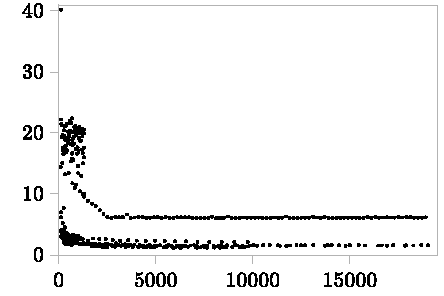
\includegraphics{td-en-funcion-m}
  \end{minipage}%
  \begin{minipage}{.5\linewidth}
    \centering
    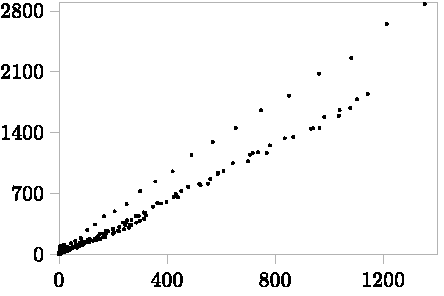
\includegraphics{t-en-funcion-d}
  \end{minipage}
  \caption{A la izquierda se muestra el gráfico de $t(G)/d(G)$ en función de $|E(G)|$, mientras que la derecha se muestra el gráfico de $t(G)/1000$ en función de $d(G)/1000$.}\label{fig:t/d-en-funcion-m}
\end{figure}



\chapter{Conclusiones y posibilidades de mejora}
\label{sec:final}

En este trabajo implementamos la estructura $h$-grafo en el lenguaje de programación \CPP.  Para esta implementación, utilizamos las estructuras estándar del lenguaje, mostrando la factibilidad del diseño de estructuras complejas y modulares.  Para lograr esta modularidad, tuvimos que hacer un uso extensivo de los iteradores, lo que nos permitió representar los punteros restringidos requeridos por la estructura $h$-grafo. Además, diseñamos nuestros propios iteradores, que nos posibilitaron brindar una interfaz eficiente con acceso en $O(1)$ a los distintos elementos del grafo, sin mostrar la estructura interna al usuario.  Más aún, mostramos que dichos iteradores cumplen con las especificaciones requeridas por el lenguaje.

Como ejemplo de uso de la nuestra implementación, escribimos un programa para encontrar los triángulos en un grafo.  De esta forma, pudimos verificar la corrección y eficiencia de la implementación.  La experimentación nos permitió concluir que la estructura es eficiente para grafos ralos, verificando empíricamente los resultados teóricos de \cite{LinSoulignacSzwarcfiterTCS2012}.

Más allá de nuestros avances, quedan algunas posibilidades de mejora que fueron excluidos del alcance de nuestro trabajo.  Podemos mencionar dos de las características más importantes que son requeridas por algunos algoritmos de~\cite{LinSoulignacSzwarcfiterTCS2012}.  Primero, sería deseable disponer de funcionalidad que permita modificar la información asociada a un vértice, sin recurrir a variables mutables.  Segundo, conviene tener una extensión que permita almacenar información en las aristas.  De esta forma, se podría almacenar el conjunto $N(vw) = N(v) \cap N(w)$ a fin de poder pos-procesarlo de forma conveniente.  Finalmente, también sería deseable implementar la variante dirigida del $h$-grafo.

En cuanto a los resultados experimentales, queda como trabajo futuro el análisis del $h$-grafo para representar grafos de gran escala.  En particular, sería deseable analizar la eficiencia empírica en comparación con otros algoritmos existentes.

\backmatter

\bibliographystyle{plain}
\bibliography{biblio}

\todos


\end{document}
